\documentclass{article}
\usepackage[margin=1in]{geometry}
\usepackage{enumitem}
\usepackage{titlesec}
\usepackage{xcolor}
\usepackage{fontspec}
\usepackage{setspace}
\usepackage{parskip}
\usepackage{graphicx}
\usepackage{fancyhdr}
\usepackage{tcolorbox}
\usepackage{array}
\usepackage{booktabs}
\usepackage{hyperref}
\usepackage{float}

\definecolor{primarycolor}{RGB}{70, 130, 180} % Steel Blue
\definecolor{secondarycolor}{RGB}{245, 245, 245} % Light Grey
\definecolor{accentcolor}{RGB}{255, 140, 0} % Dark Orange
\definecolor{darkblue}{RGB}{0, 0, 139} % Dark Blue

\hypersetup{
    colorlinks=true,
    linkcolor=primarycolor,
    urlcolor=accentcolor,
    citecolor=primarycolor,
}

\titleformat{\section}
  {\normalfont\Large\bfseries\color{primarycolor}}
  {\thesection.}{0.5em}{}[\titlerule]

\pagestyle{fancy}
\fancyhf{}
\fancyhead[L]{The Oaklaura Bike Cooperative}
\fancyhead[R]{CS340 - Introduction to Databases, Spring 2025}
\fancyfoot[C]{\thepage}
\renewcommand{\headrulewidth}{1pt}
\renewcommand{\headrule}{\hbox to\headwidth{\color{primarycolor}\leaders\hrule height \headrulewidth\hfill}}

\setlist[itemize]{leftmargin=*, label={\color{accentcolor}$\bullet$}}
\begin{document}
\begin{center}
\large\textcolor{primarycolor}{\textbf{Project Group \#1: Team Oaklaura}}\\[0.3cm]
\large\textbf{Grant Wu and Jessica Ramirez}\\[0.3cm]
\huge\textbf{Project Step 6 - Final}\\[0.5cm]

\large\textbf{URL to Oaklaura Bike Co-Op UI:}\\[0.5cm]
\large\href{http://classwork.engr.oregonstate.edu:7013/}{\textcolor{darkblue}{\textbf{http://classwork.engr.oregonstate.edu:7013/}}}\\[1.25cm]
\end{center}
%%%%%%%%%%%%%%%%%%%%%%%%%%%%%%%%%%%%%%%%%%%%%%%%%%%%%%%%%%%%%
%%%%%%%%%%%%%%.                   SECTION 1: Executive Summary                      %%%%%%%%%%%%%%%%%
%%%%%%%%%%%%%%%%%%%%%%%%%%%%%%%%%%%%%%%%%%%%%%%%%%%%%%%%%%%%%
\section{Executive Summary}
%%%%%%%%%%%%%%%%%%%%%%%%%%%%%%%%%%%%%%%%%%%%%%%%%%%%%%%%%%%%%
\begin{tcolorbox}[colback=secondarycolor, colframe=primarycolor, title=\textbf{Reflection on Major Changes Throughout Project}]

Over the course of 11 weeks, our team (Grant Wu and Jessica Ramirez) developed a full-stack web application underpinned by a normalized relational database. This project followed a multi-phase structure that allowed us to build iteratively while incorporating continuous feedback from teaching assistants and peer reviewers.

\vspace{0.2cm}

The project began with the design of a schema representing a real-world bike co-op scenario. Our initial design featured five entities: StorePersonnel, Customers, Bikes, RepairReports, and SalesReports. Early feedback helped us identify normalization issues, prompting the addition of a sixth entity—Contacts—to eliminate redundancy and ensure compliance with 3rd Normal Form (3NF). Following schema finalization, we translated the design into SQL through structured DDL and DML scripts. We replaced hardcoded foreign keys with subqueries and corrected naming inconsistencies in foreign key attributes to improve clarity and maintain consistency.

\vspace{0.2cm}

Subsequent phases focused on UI development, beginning with static data display and evolving into a fully interactive interface. We implemented CRUD operations—Create, Read, Update, and Delete—for both the RepairReports (our M:M relationship intersection table) and Contacts tables. The Contacts table was chosen to demonstrate the ON DELETE CASCADE behavior defined in the DDL.sql file, specifically, how deleting a contact cascades the deletion to related records, thereby preventing deletion anomalies. A key design decision was to limit CUD functionality to two tables to maintain a clean, focused interface that exceeded project requirements without over-complication. To support demonstration and testing, we also added a Reset button that drops and reinitializes all tables with default data.

\vspace{0.2cm}

Major refinements based on feedback included:
\vspace{0.1cm}
\begin{itemize}
    \item Consistent column aliases for readability
    \item Dropdowns and updated foreign key displays using human-readable names
    \item Moving Add buttons to the top of tables for accessibility
    \item Standardized date formatting
    \item Improved UI layout and centering
    \item Bug fixes in update forms and dropdown population
    \item Confirmation popups preceding delete and reset actions
\end{itemize}

\vspace{0.2cm}

Overall, our application demonstrates not only the core of database design and web integration, but also a commitment to ease of use, aesthetic appeal and incorporation of independent feedback.
\end{tcolorbox}

%%%%%%%%%%%%%%%%%%%%%%%%%%%%%%%%%%%%%%%%%%%%%%%%%%%%%%%%%%%%%
%%%%%%%%%%%%%.                   SECTION 2: Overview                    %%%%%%%%%%%%%%%%%%%%%%%%
%%%%%%%%%%%%%%%%%%%%%%%%%%%%%%%%%%%%%%%%%%%%%%%%%%%%%%%%%%%%%
\section{Project Overview: The Oaklaura Bike Cooperative}

\begin{tcolorbox}[colback=secondarycolor, colframe=primarycolor, arc=5mm]
\begingroup
The Oaklaura Bike Cooperative is a non-profit organization that accepts donations of old or broken bicycles, refurbishes them, and then sells them at an affordable price. The co-op sees 50-100 bicycles enter and exit their doors on a monthly basis. Due to limited funding, the co-op operates with a small team of 10 employees and relies heavily on volunteers to assist with bicycle repairs. At the current time there are about 100 volunteers that donate their time, and this is expected to grow over the course of the next five years. The co-op’s limited funding also requires they use a basic POS system that can only process one bike sale at a time, setting a limit of one bike per sales order. The co-op brings in on average between \$10,000 and \$25,000 per month, and most of this revenue is used to support the small team of dedicated employees as well as to provide community engagement events. 

\vspace{0.2cm}

Store personnel consist of both volunteers and employees. Most volunteers are not experienced bike mechanics, so they often can't fully repair a bike during the few hours the co-op is open for volunteer work. To maintain continuity and organization, volunteers are expected to repair what they can during their shift and document their progress in a report the same day the work was performed. This allows the next volunteer and/or employee to review the logs and continue the work where the previous one left off. Sometimes volunteers engage in non-bike specific work, such as cleaning and fixing stock parts such as cassettes, wheels and derailleurs, which gets documented in these repair reports as well. Once a volunteer believes a bike is fully repaired, a trained employee inspects it to ensure it meets safety standards before placing it on the sales floor. Once there, a bike can be sold, a transaction which is tracked through a sales report. 

\vspace{0.2cm}

Historically, the co-op tracked repair progress and sales using handwritten notecards stored in a filing cabinet. However, as the organization grows, this system has become increasingly difficult to manage. Implementing a database would be an ideal solution for organizing and sharing information between volunteers and employees about the status of each bicycle, as well as for tracking the inventory and sales history of the ever expanding co-op.

\endgroup
\end{tcolorbox}

\vspace{0.5cm}

%%%%%%%%%%%%%%%%%%%%%%%%%%%%%%%%%%%%%%%%%%%%%%%%%%%%%%%%%%%%%
%%%%%%%%%%%.                   SECTION 3: Database Outline                       %%%%%%%%%%%%%%%%%%%%%
%%%%%%%%%%%%%%%%%%%%%%%%%%%%%%%%%%%%%%%%%%%%%%%%%%%%%%%%%%%%%
\section{Database Overview}

%%%%%%%%%%%%%%%%.%                       BIKES                         %%%%%%%%%%%%%%%%%%%%%%%%%
\begin{tcolorbox}[colback=secondarycolor, colframe=primarycolor, title=\textbf{Bikes Table}]
Contains details on a particular bike that resides within the co-op.
\vspace{0.2cm}

\begin{itemize}
  \item \textbf{bikeID [PK]:} int, not NULL, auto\_increment
  \item \textbf{color:} enum(`Black', `White', `Red', `Blue', `Green', `Pink', `Purple', `Yellow', `Orange', `Silver', `Other'), not NULL 
  \item \textbf{style:} enum(`Mountain', `Road', `Fat', `Hybrid', `Enduro', `BMX', `Cruiser', `Kids', `Electric'), not NULL
  \item \textbf{brand:} varchar(45), not NULL
  \item \textbf{status:} enum(`In Repair', `In Review', `For Sale', `Sold'), not NULL
  \item \textbf{dateReceived:} date, not NULL
\end{itemize}
\vspace{0.2cm}

\textbf{Relationships:}
\vspace{0.2cm}
\begin{itemize}
  \item M:M relationship between Bikes and StorePersonnel is implemented with bikeID and personnelID as FK's within both RepairReports and within SalesReports.
  \item 1:1 relationship between Bikes and SalesReports is implemented by bikeID as a FK within SalesReports. \textit{Note: due to our outdated POS system, only one bike can be sold at a time (i.e. only one Bike can appear on each SalesReport).}
  \item 1:M relationship between Bikes and RepairReports is implemented with bikeID as a FK within RepairReports.
\end{itemize}
\end{tcolorbox}

\vspace{0.5cm}

%%%%%%%%%%%%%%%.%                       STOREPERSONNEL                         %%%%%%%%%%%%%%%%%%%%%%%
\begin{tcolorbox}[colback=secondarycolor, colframe=primarycolor, title=\textbf{StorePersonnel Table}]
Holds information on store employees and volunteers that work within the co-op.
\vspace{0.2cm}

\begin{itemize}
  \item \textbf{personnelID [PK]:} int, not NULL, auto\_increment
  \item \textbf{contactID [FK - Contacts]:} int, not NULL
  \item \textbf{role:} enum(`Employee', `Volunteer'), not NULL
\end{itemize}
\vspace{0.2cm}

\textbf{Relationships:}
\vspace{0.2cm}
\begin{itemize}
  \item M:M relationship between StorePersonnel and Bikes is implemented with bikeID and personnelID as FK's within both RepairReports and within SalesReports.
  \item 1:M relationship between StorePersonnel and RepairReports is implemented with personnelID as a FK within RepairReports.
    \item 1:1 relationship between StorePersonnel and Contacts is implemented with contactID as a FK within StorePersonnel.
\end{itemize}
\end{tcolorbox}

\vspace{0.5cm}

%%%%%%%%%%%%%%%.%                       CUSTOMERS                         %%%%%%%%%%%%%%%%%%%%%%%
\begin{tcolorbox}[colback=secondarycolor, colframe=primarycolor, title=\textbf{Customers Table}]
Holds information relating to existing and potential customers.
\vspace{0.2cm}

\begin{itemize}
  \item \textbf{customerID [PK]:} int, not NULL, auto\_increment
  \item \textbf{contactID [FK - Contacts]:} int, not NULL
  \item \textbf{receiveNewsletter:} tinyint, not NULL, DEFAULT = 0 (false)
\end{itemize}
\vspace{0.2cm}

\textbf{Relationships:}
\vspace{0.2cm}
\begin{itemize}
  \item 1:M relationship between Customers and SalesReports is implemented with customerID as a FK inside of SalesReports.
  \item 1:1 relationship between Customers and Contacts is implemented with contactID as a FK within Customers.
\end{itemize}
\end{tcolorbox}

\vspace{0.5cm}

%%%%%%%%%%%%%%%.%                       REPAIRREPORTS                        %%%%%%%%%%%%%%%%%%%%%%%
\begin{tcolorbox}[colback=secondarycolor, colframe=primarycolor, title=\textbf{RepairReports Table}]
Holds repair information performed on a particular bikes (Bikes\_StorePersonnel Intersection Table that includes additional repair information).
\vspace{0.2cm}

\begin{itemize}
  \item \textbf{repairID [PK]:} int, not NULL, auto\_increment
  \item \textbf{personnelID [FK - StorePersonnel]:} int, not NULL
  \item \textbf{bikeID [FK - Bikes]:} int
  \item \textbf{dateRepaired:} datetime, not NULL
  \item \textbf{hoursSpent:} decimal(4,2), not NULL
  \item \textbf{description:} varchar(255), not NULL
\end{itemize}
\vspace{0.2cm}

\textbf{Relationships:}
\vspace{0.2cm}
\begin{itemize}
  \item 1:M relationship between RepairReports and StorePersonnel is implemented with personnelID as a FK inside RepairReports.
  \item 1:M relationship between RepairReports and Bikes is implemented with bikeID as a FK inside RepairReports.
\end{itemize}
\end{tcolorbox}

\vspace{0.5cm}

%%%%%%%%%%%%%%%%.%                       SALESREPORTS                        %%%%%%%%%%%%%%%%%%%%%%%%
\begin{tcolorbox}[colback=secondarycolor, colframe=primarycolor, title=\textbf{SalesReports Table}]
Holds information pertaining to the sale of a particular bike.
\vspace{0.2cm}

\begin{itemize}
  \item \textbf{salesID [PK]:} int, not NULL, auto\_increment
  \item \textbf{bikeID [FK - Bikes]:} int, not NULL, unique
  \item \textbf{customerID [FK - Customers]:} int, not NULL
  \item \textbf{dateSold:} date, not NULL
  \item \textbf{price:} decimal(5,2), not NULL
\end{itemize}
\vspace{0.2cm}

\textbf{Relationships:}
\vspace{0.2cm}
\begin{itemize}
  \item 1:1 relationship between Bikes and SalesReports is implemented by bikeID as a FK within SalesReports. \textit{Note: due to our outdated POS system, only one bike can be sold at a time (i.e. only one Bike can appear on each SalesReport).}
  \item 1:M relationship between SalesReports and Customers is implemented with customerID as a FK within SalesReports.
\end{itemize}
\end{tcolorbox}

\vspace{0.5cm}

%%%%%%%%%%%%%%%.%                       CONTACTS                         %%%%%%%%%%%%%%%%%%%%%%%
\begin{tcolorbox}[colback=secondarycolor, colframe=primarycolor, title=\textbf{Contacts Table}]
Holds contact information for any person in the system (both service providers and service recipients).
 
 \vspace{0.2cm}

\begin{itemize}
  \item \textbf{contactID [PK]:} int, not NULL, auto\_increment
  \item \textbf{firstName:} varchar(45) not NULL
  \item \textbf{lastName:} varchar(45) not NULL
  \item \textbf{phone:} varchar(45), not NULL
  \item \textbf{email:} varchar(100), not NULL, UNIQUE
\end{itemize}
\vspace{0.2cm}

\textbf{Relationships:}
\vspace{0.2cm}
\begin{itemize}
   \item 1:1 relationship between Contacts and StorePersonnel is implemented with contactID as a FK within Customers.
   \item 1:1 relationship between Contacts and Customers is implemented with contactID as a FK within Customers.
\end{itemize}
\end{tcolorbox}

\vspace{0.5cm}

%%%%%%%%%%%%%%%%%%%%%%%%%%%%%%%%%%%%%%%%%%%%%%%%%%%%%%%%%%%%%
%%%%%%%%%%%%%%.                   SECTION 4: ERD                       %%%%%%%%%%%%%%%%%%%%%%%%%
%%%%%%%%%%%%%%%%%%%%%%%%%%%%%%%%%%%%%%%%%%%%%%%%%%%%%%%%%%%%%
\section{Entity-Relationship Diagram}

\begin{tcolorbox}[colback=secondarycolor, colframe=primarycolor, arc=5mm]

\begin{center}
\vspace{0.5cm}
 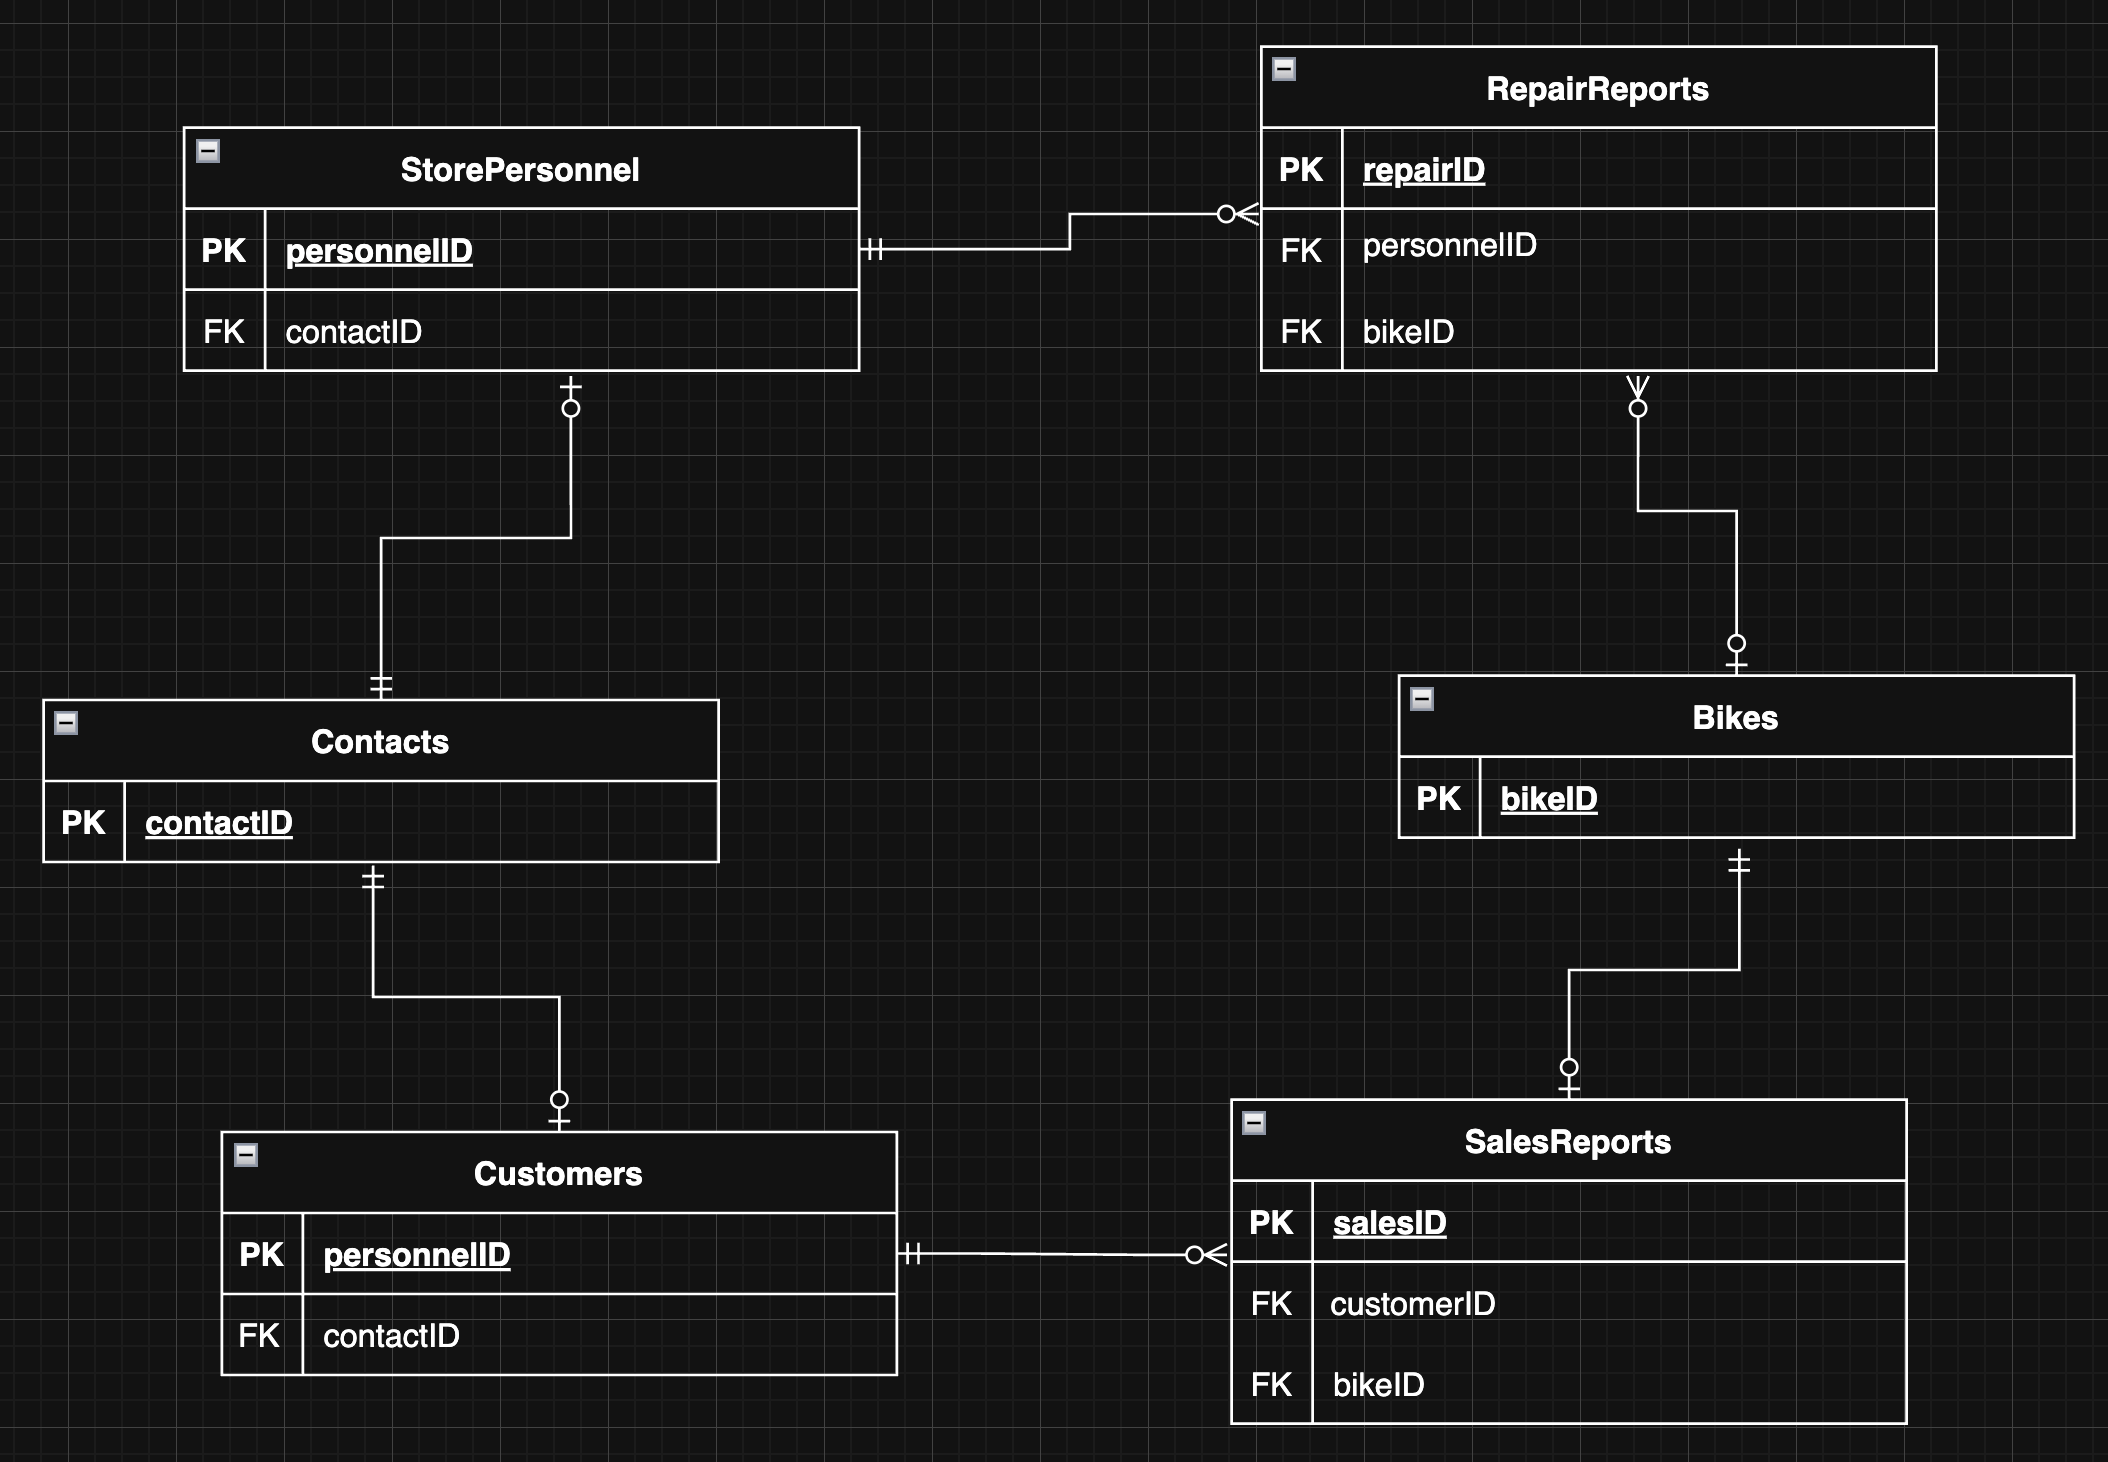
\includegraphics[width=0.9\textwidth]{ERD.png}
\end{center}
\end{tcolorbox}

\vspace{0.5cm}

%%%%%%%%%%%%%%%%%%%%%%%%%%%%%%%%%%%%%%%%%%%%%%%%%%%%%%%%%%%%%
%%%%%%%%%%%%%%.                   SECTION 5: Schema                       %%%%%%%%%%%%%%%%%%%%%%%
%%%%%%%%%%%%%%%%%%%%%%%%%%%%%%%%%%%%%%%%%%%%%%%%%%%%%%%%%%%%%
\section{Schema Diagram}

\begin{tcolorbox}[colback=secondarycolor, colframe=primarycolor, arc=5mm]

\begin{center}
\vspace{0.5cm}
 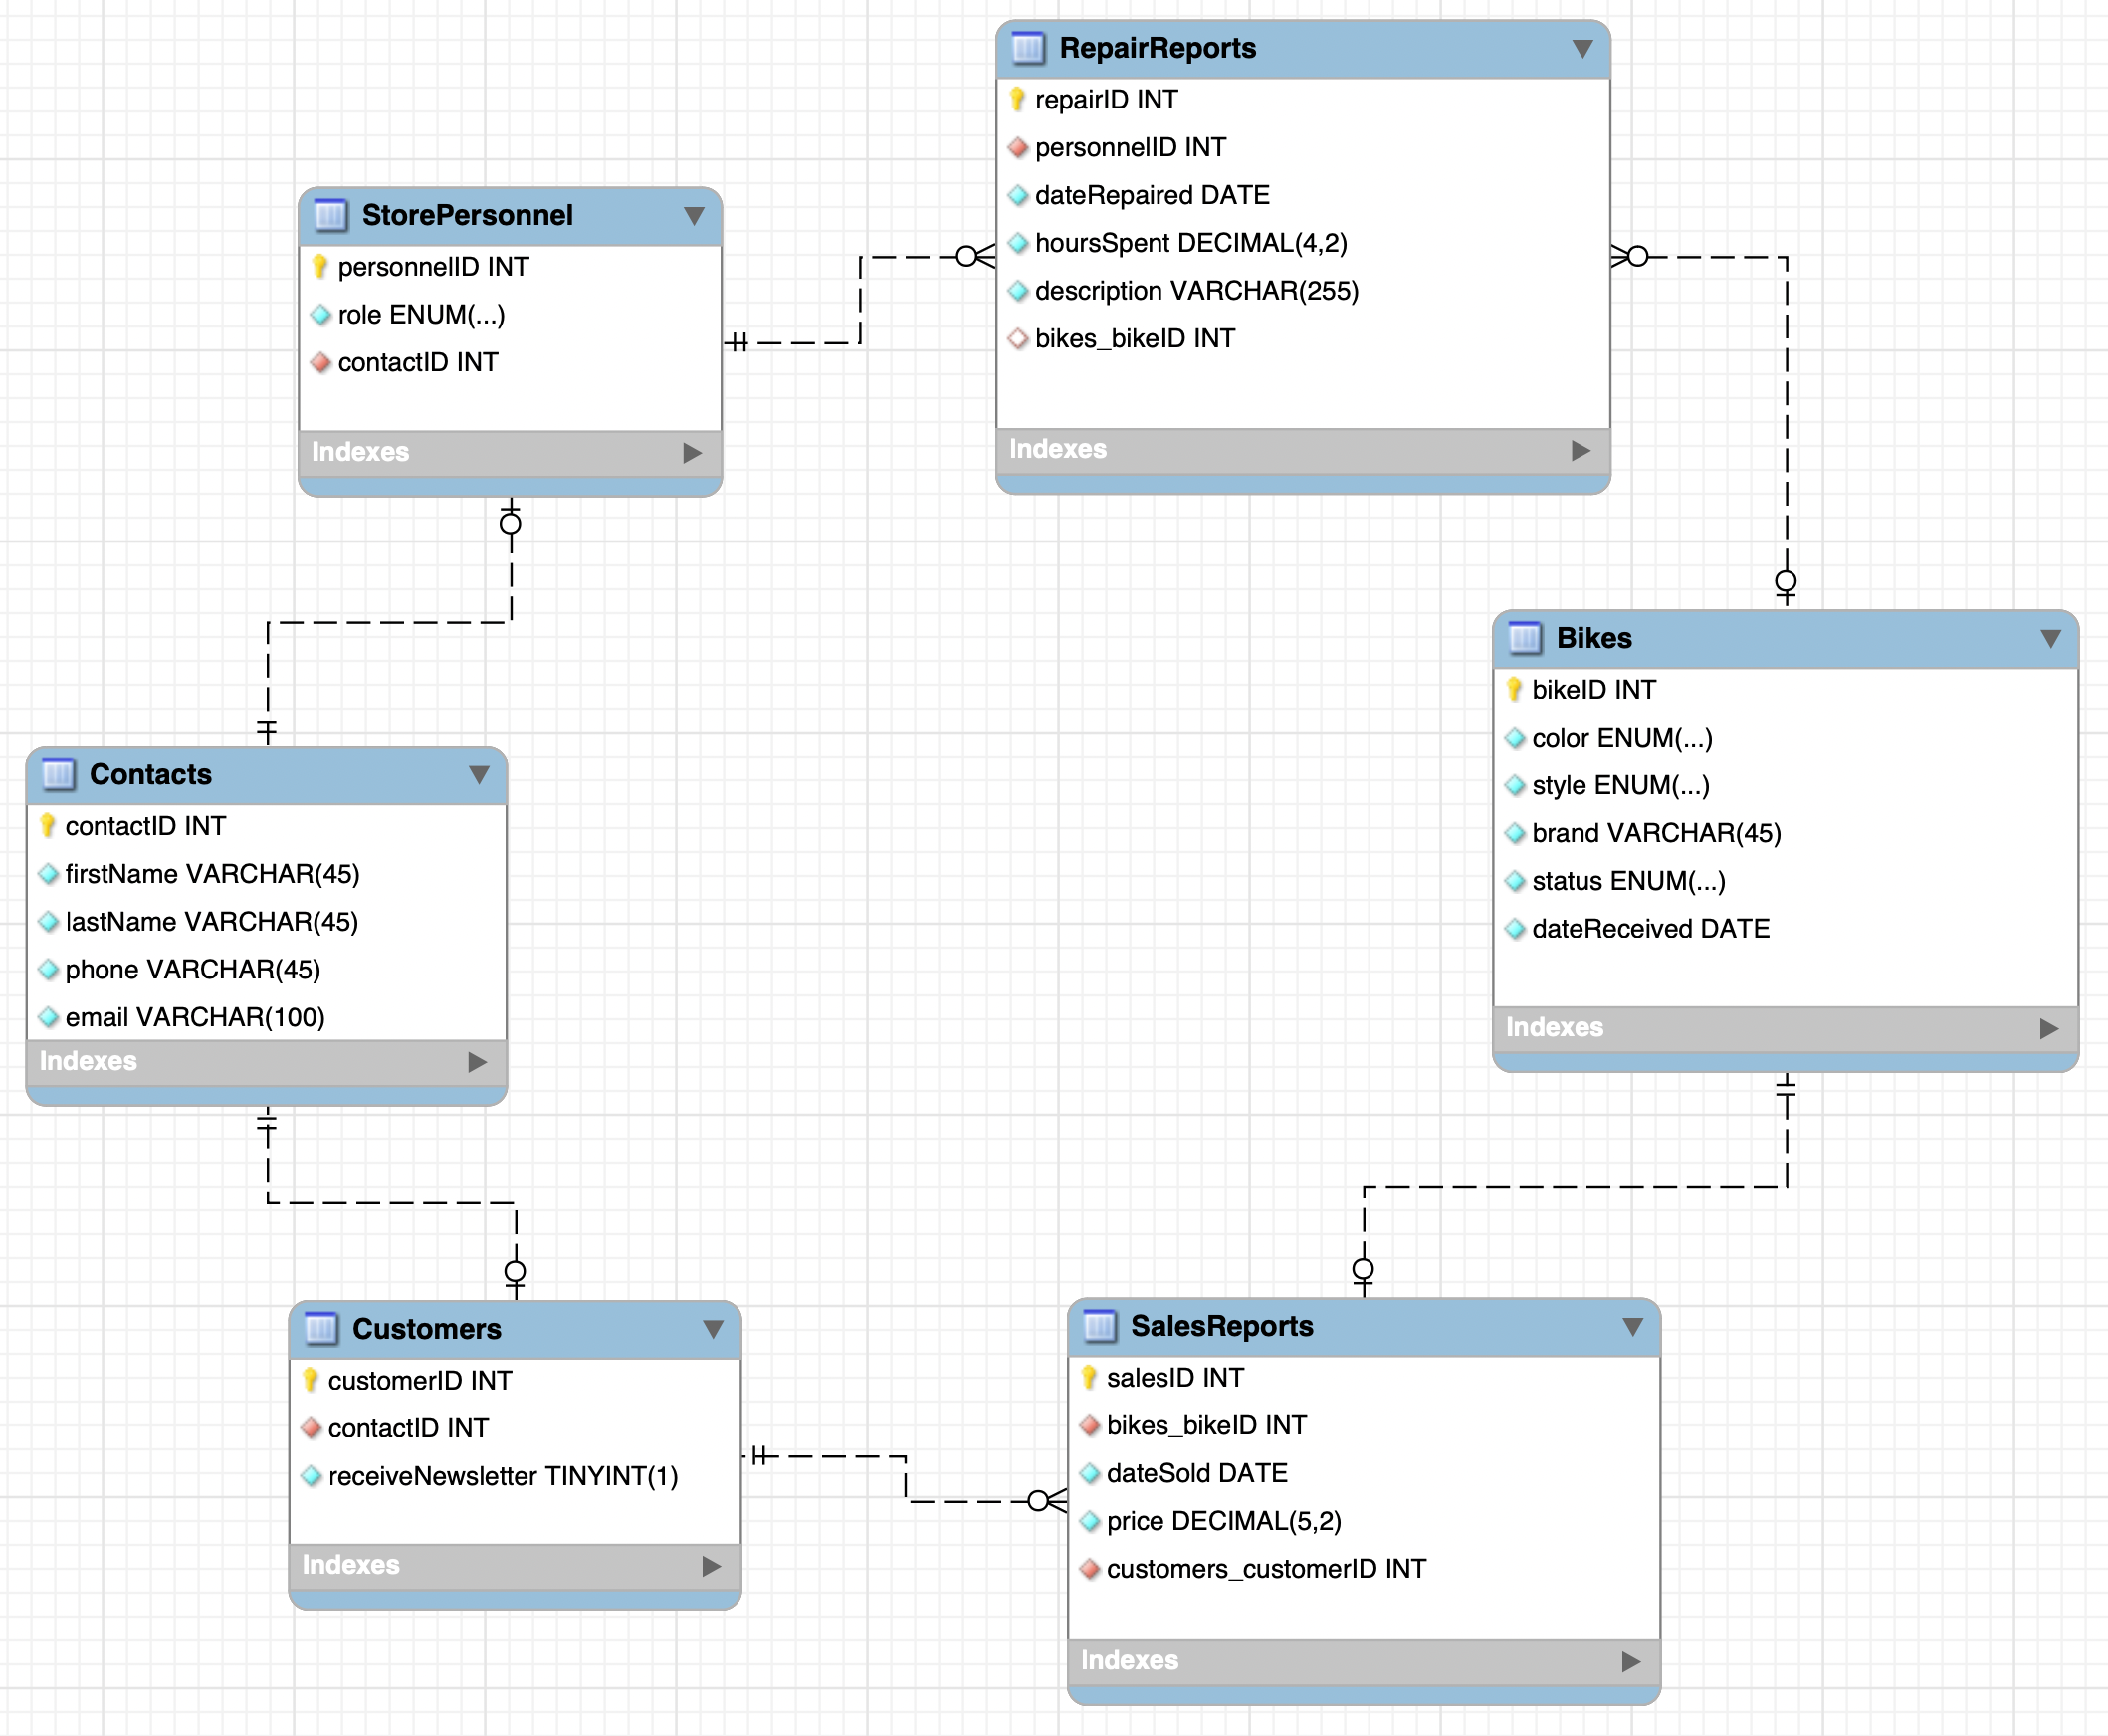
\includegraphics[width=0.9\textwidth]{Schema.png}
\end{center}
\end{tcolorbox}

\vspace{0.5cm}

%%%%%%%%%%%%%%%%%%%%%%%%%%%%%%%%%%%%%%%%%%%%%%%%%%%%%%%%%%%%%
%%%%%%%%%%%%%.                   SECTION 6: Sample Data.                       %%%%%%%%%%%%%%%%%%%%%
%%%%%%%%%%%%%%%%%%%%%%%%%%%%%%%%%%%%%%%%%%%%%%%%%%%%%%%%%%%%%
\section{Sample Data}

\begin{figure}[H]
    \centering
    \caption{Sample data inserted into the Bikes table}
    \vspace{0.2cm}
    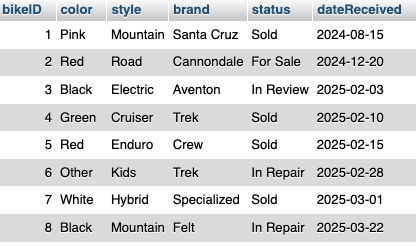
\includegraphics[width=0.5\textwidth]{Bikes.png}
    \label{fig:Bikes}
\end{figure}

\begin{figure}[H]
    \centering
    \caption{Sample data inserted into the StorePersonnel table}
    \vspace{0.2cm}
    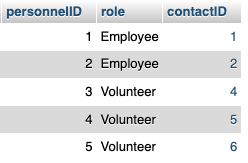
\includegraphics[width=0.5\textwidth]{StorePersonnel.png}
    \label{fig:StorePersonnel}
\end{figure}

\begin{figure}[H]
    \centering
    \caption{Sample data inserted into the Customers table}
    \vspace{0.2cm}
    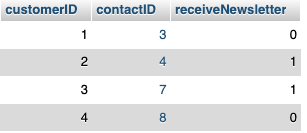
\includegraphics[width=0.5\textwidth]{Customers.png}
    \label{fig:Customers}
\end{figure}

\begin{figure}[H]
    \centering
    \caption{Sample data inserted into the RepairReports table}
    \vspace{0.2cm}
    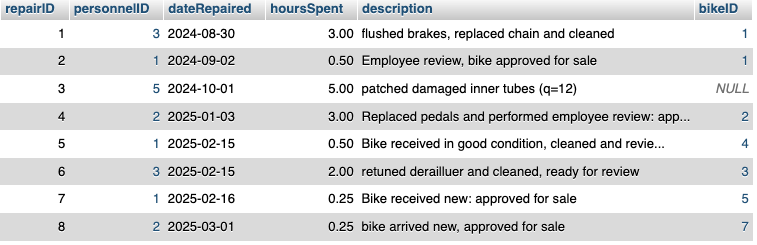
\includegraphics[width=0.5\textwidth]{RepairReports.png}
    \label{fig:RepairReports}
\end{figure}

\begin{figure}[H]
    \centering
    \caption{Sample data inserted into the SalesReports table}
    \vspace{0.2cm}
    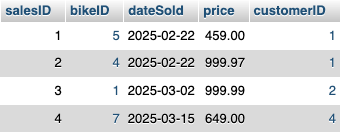
\includegraphics[width=0.5\textwidth]{SalesReports.png}
    \label{fig:SalesReports}
\end{figure}

\begin{figure}[H]
    \centering
    \caption{Sample data inserted into the Contacts table}
    \vspace{0.2cm}
    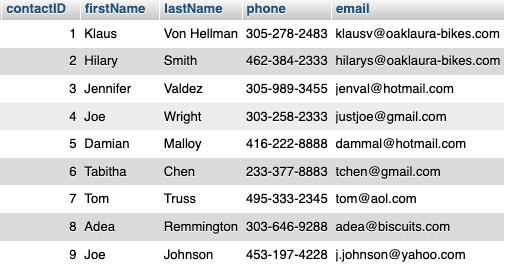
\includegraphics[width=0.5\textwidth]{Contacts.png}
    \label{fig:Contacts}
\end{figure}

%%%%%%%%%%%%%%%%%%%%%%%%%%%%%%%%%%%%%%%%%%%%%%%%%%%%%%%%%%%%%
%%%%%%%%%%%.                   SECTION 7: UI Screenshots                       %%%%%%%%%%%%%%%%%%%%%%
%%%%%%%%%%%%%%%%%%%%%%%%%%%%%%%%%%%%%%%%%%%%%%%%%%%%%%%%%%%%%
\section{UI Screen Shots}

\begin{figure}[H]
    \centering
    \caption{Read Bikes table}
    \vspace{0.2cm}
    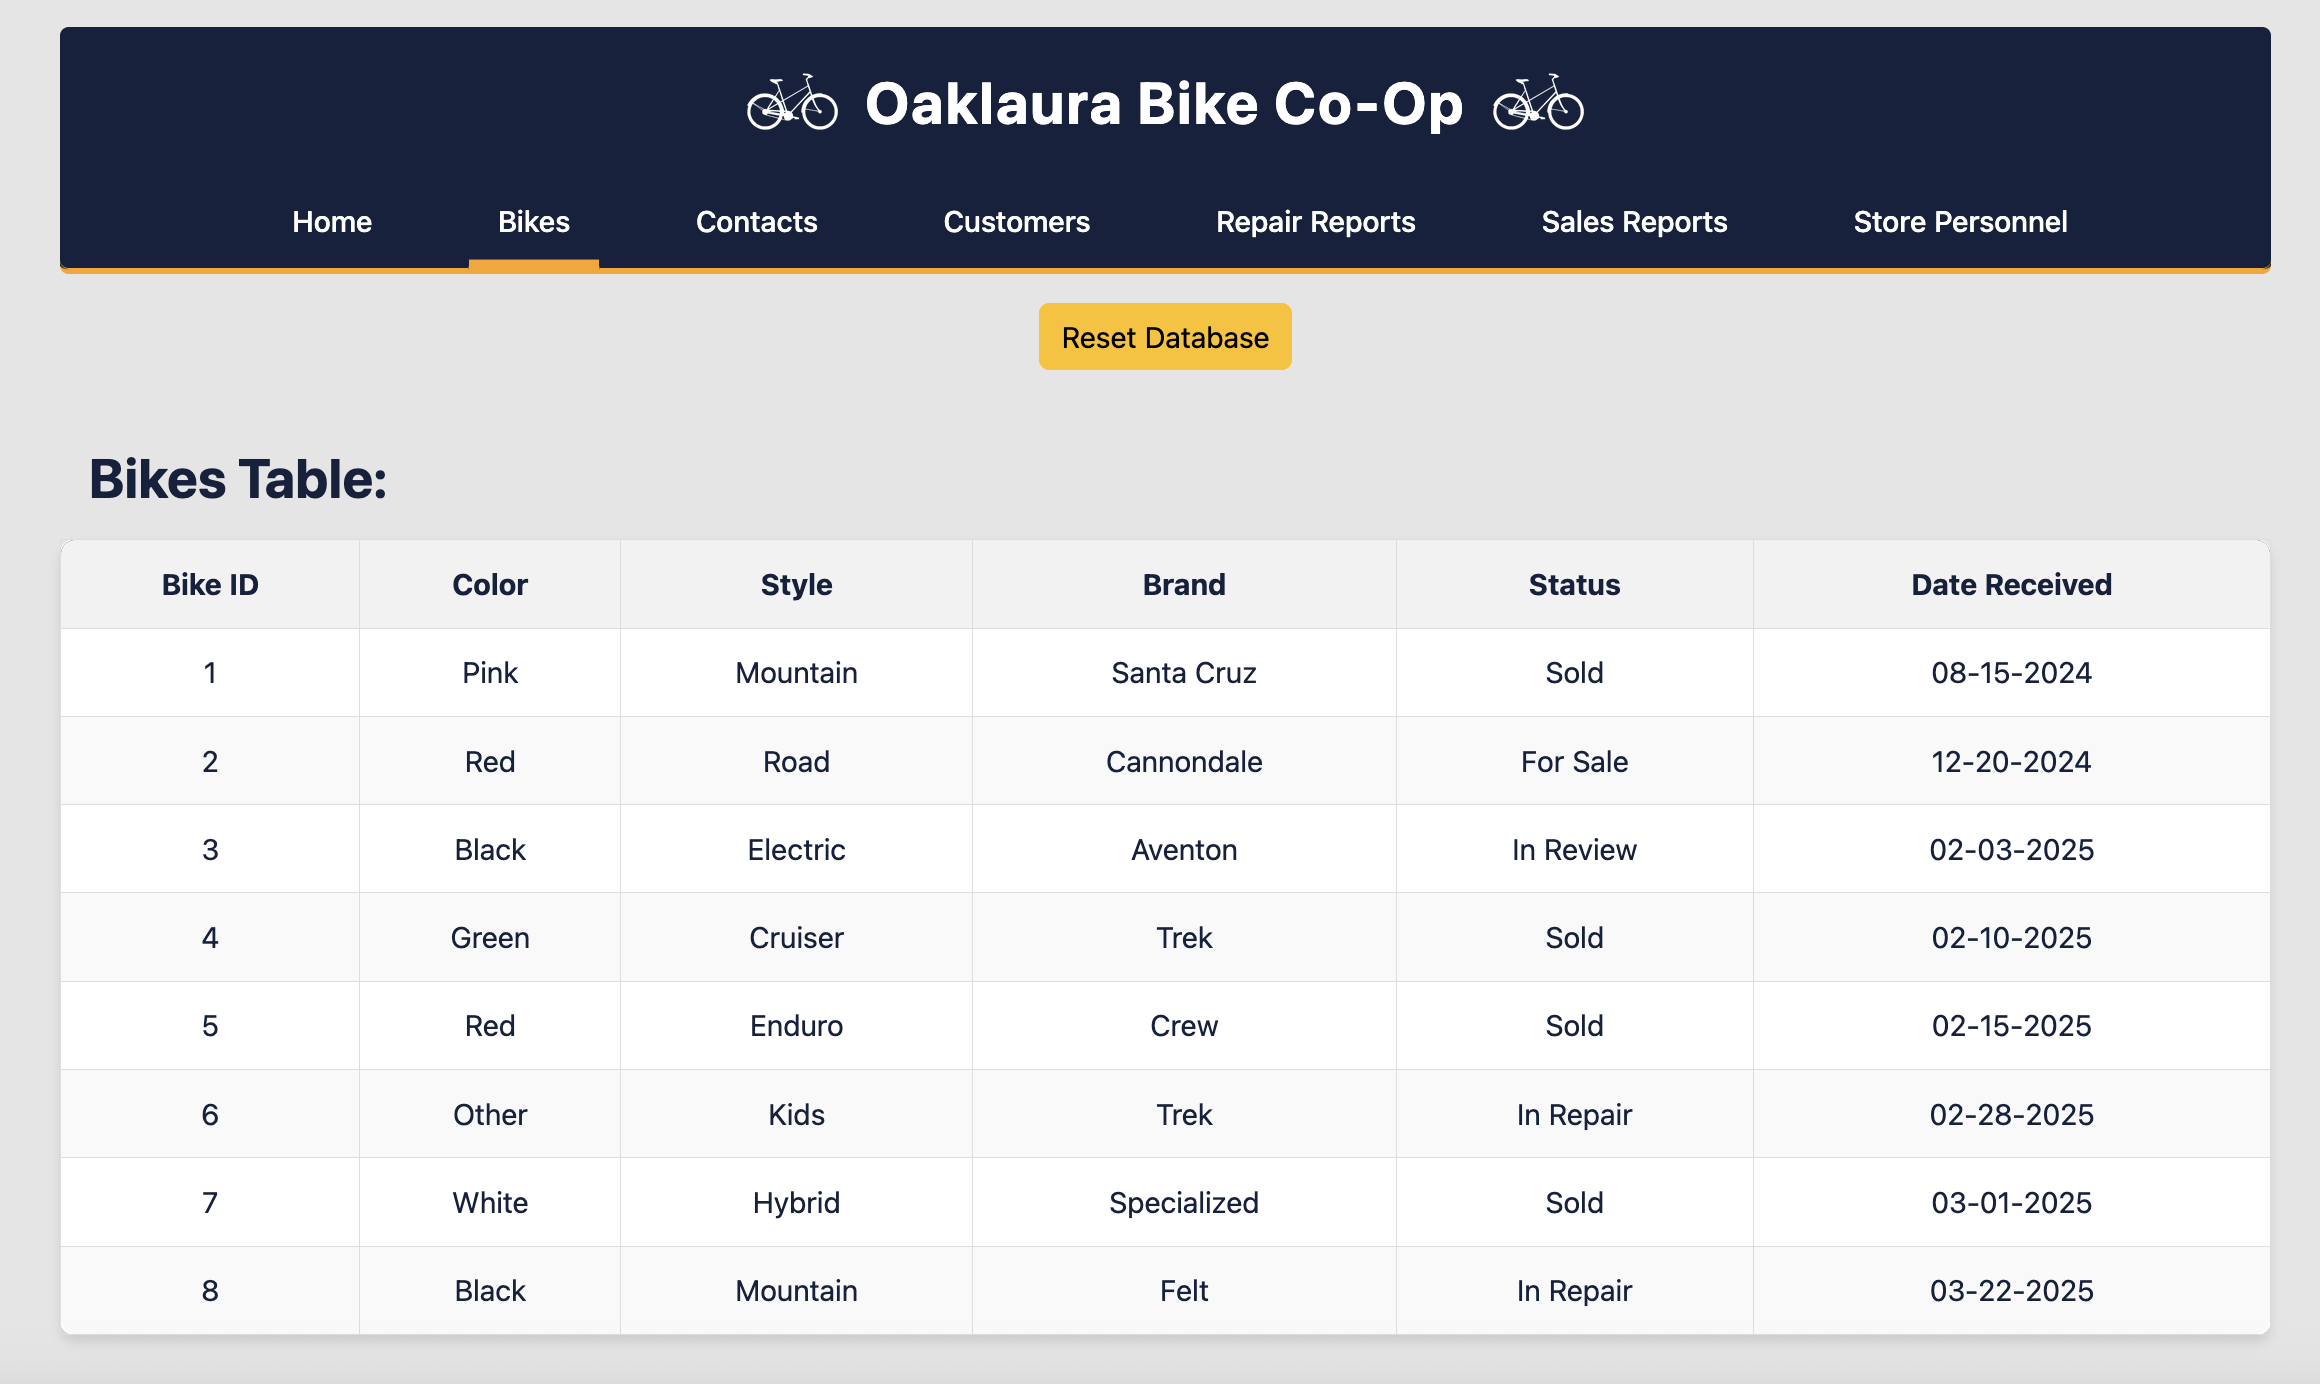
\includegraphics[width=1.0\textwidth]{UI_screenshots/Read_Bikes_Table.png}
    \label{fig:Read Bikes table}
\end{figure}

\begin{figure}[H]
    \centering
    \caption{Read Contacts table}
    \vspace{0.2cm}
    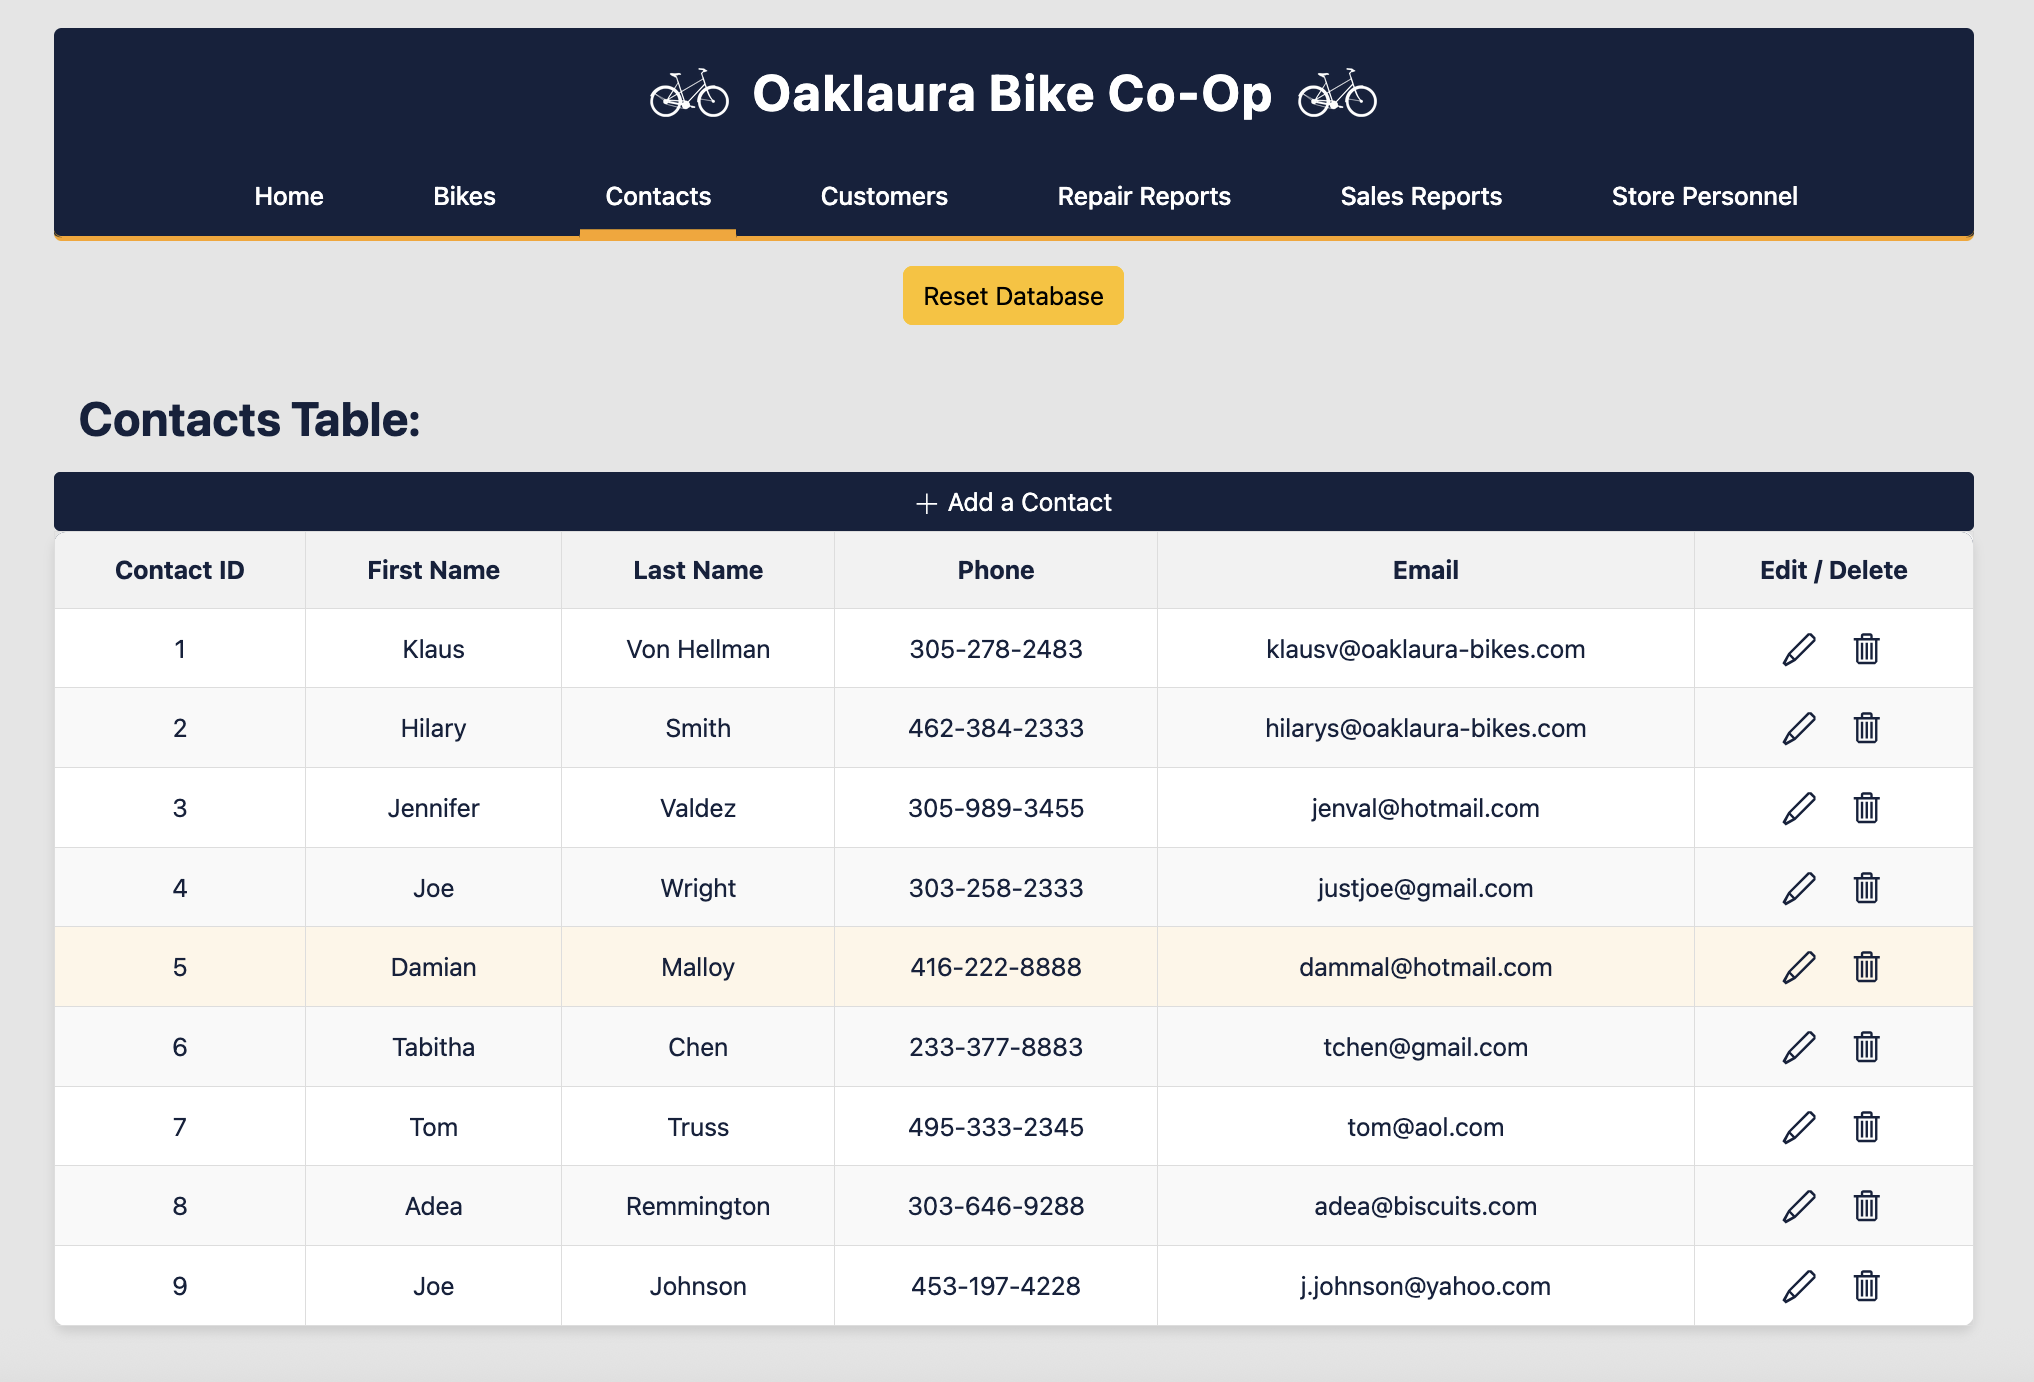
\includegraphics[width=1.0\textwidth]{UI_screenshots/Read_Contacts_Page.png}
    \label{fig:Read Contacts table}
\end{figure}

\begin{figure}[H]
    \centering
    \caption{Read Customers table}
    \vspace{0.2cm}
    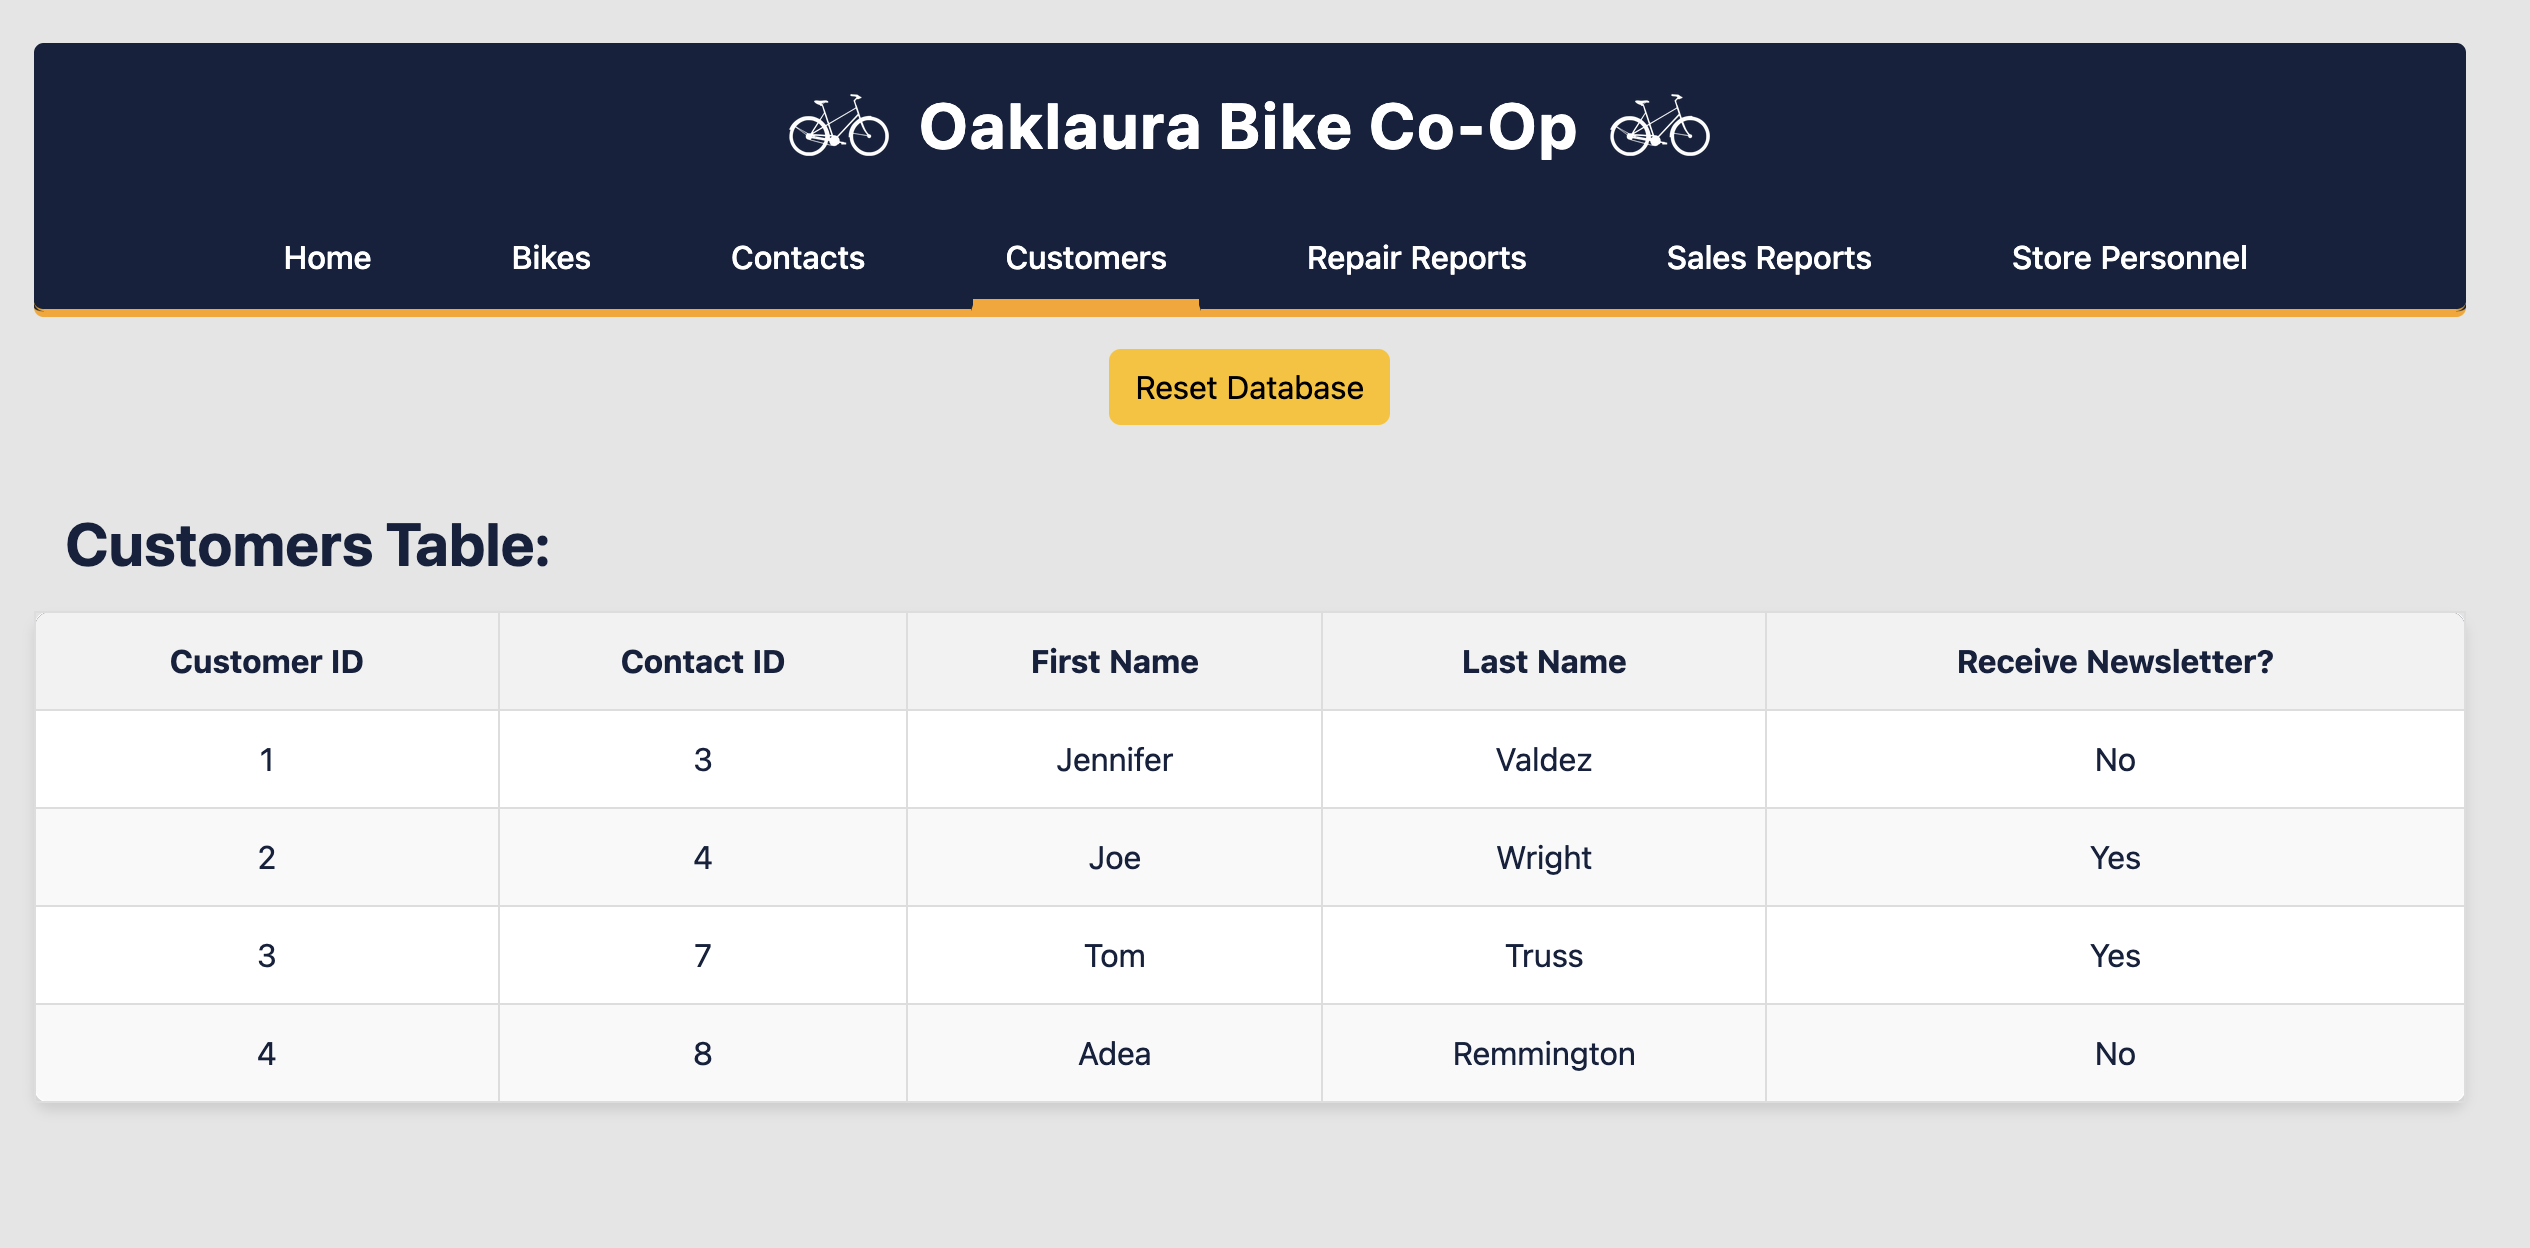
\includegraphics[width=1.0\textwidth]{UI_screenshots/Read_Customers_Table.png}
    \label{fig:Read Customers table}
\end{figure}

\begin{figure}[H]
    \centering
    \caption{Read Repair Reports table}
    \vspace{0.2cm}
    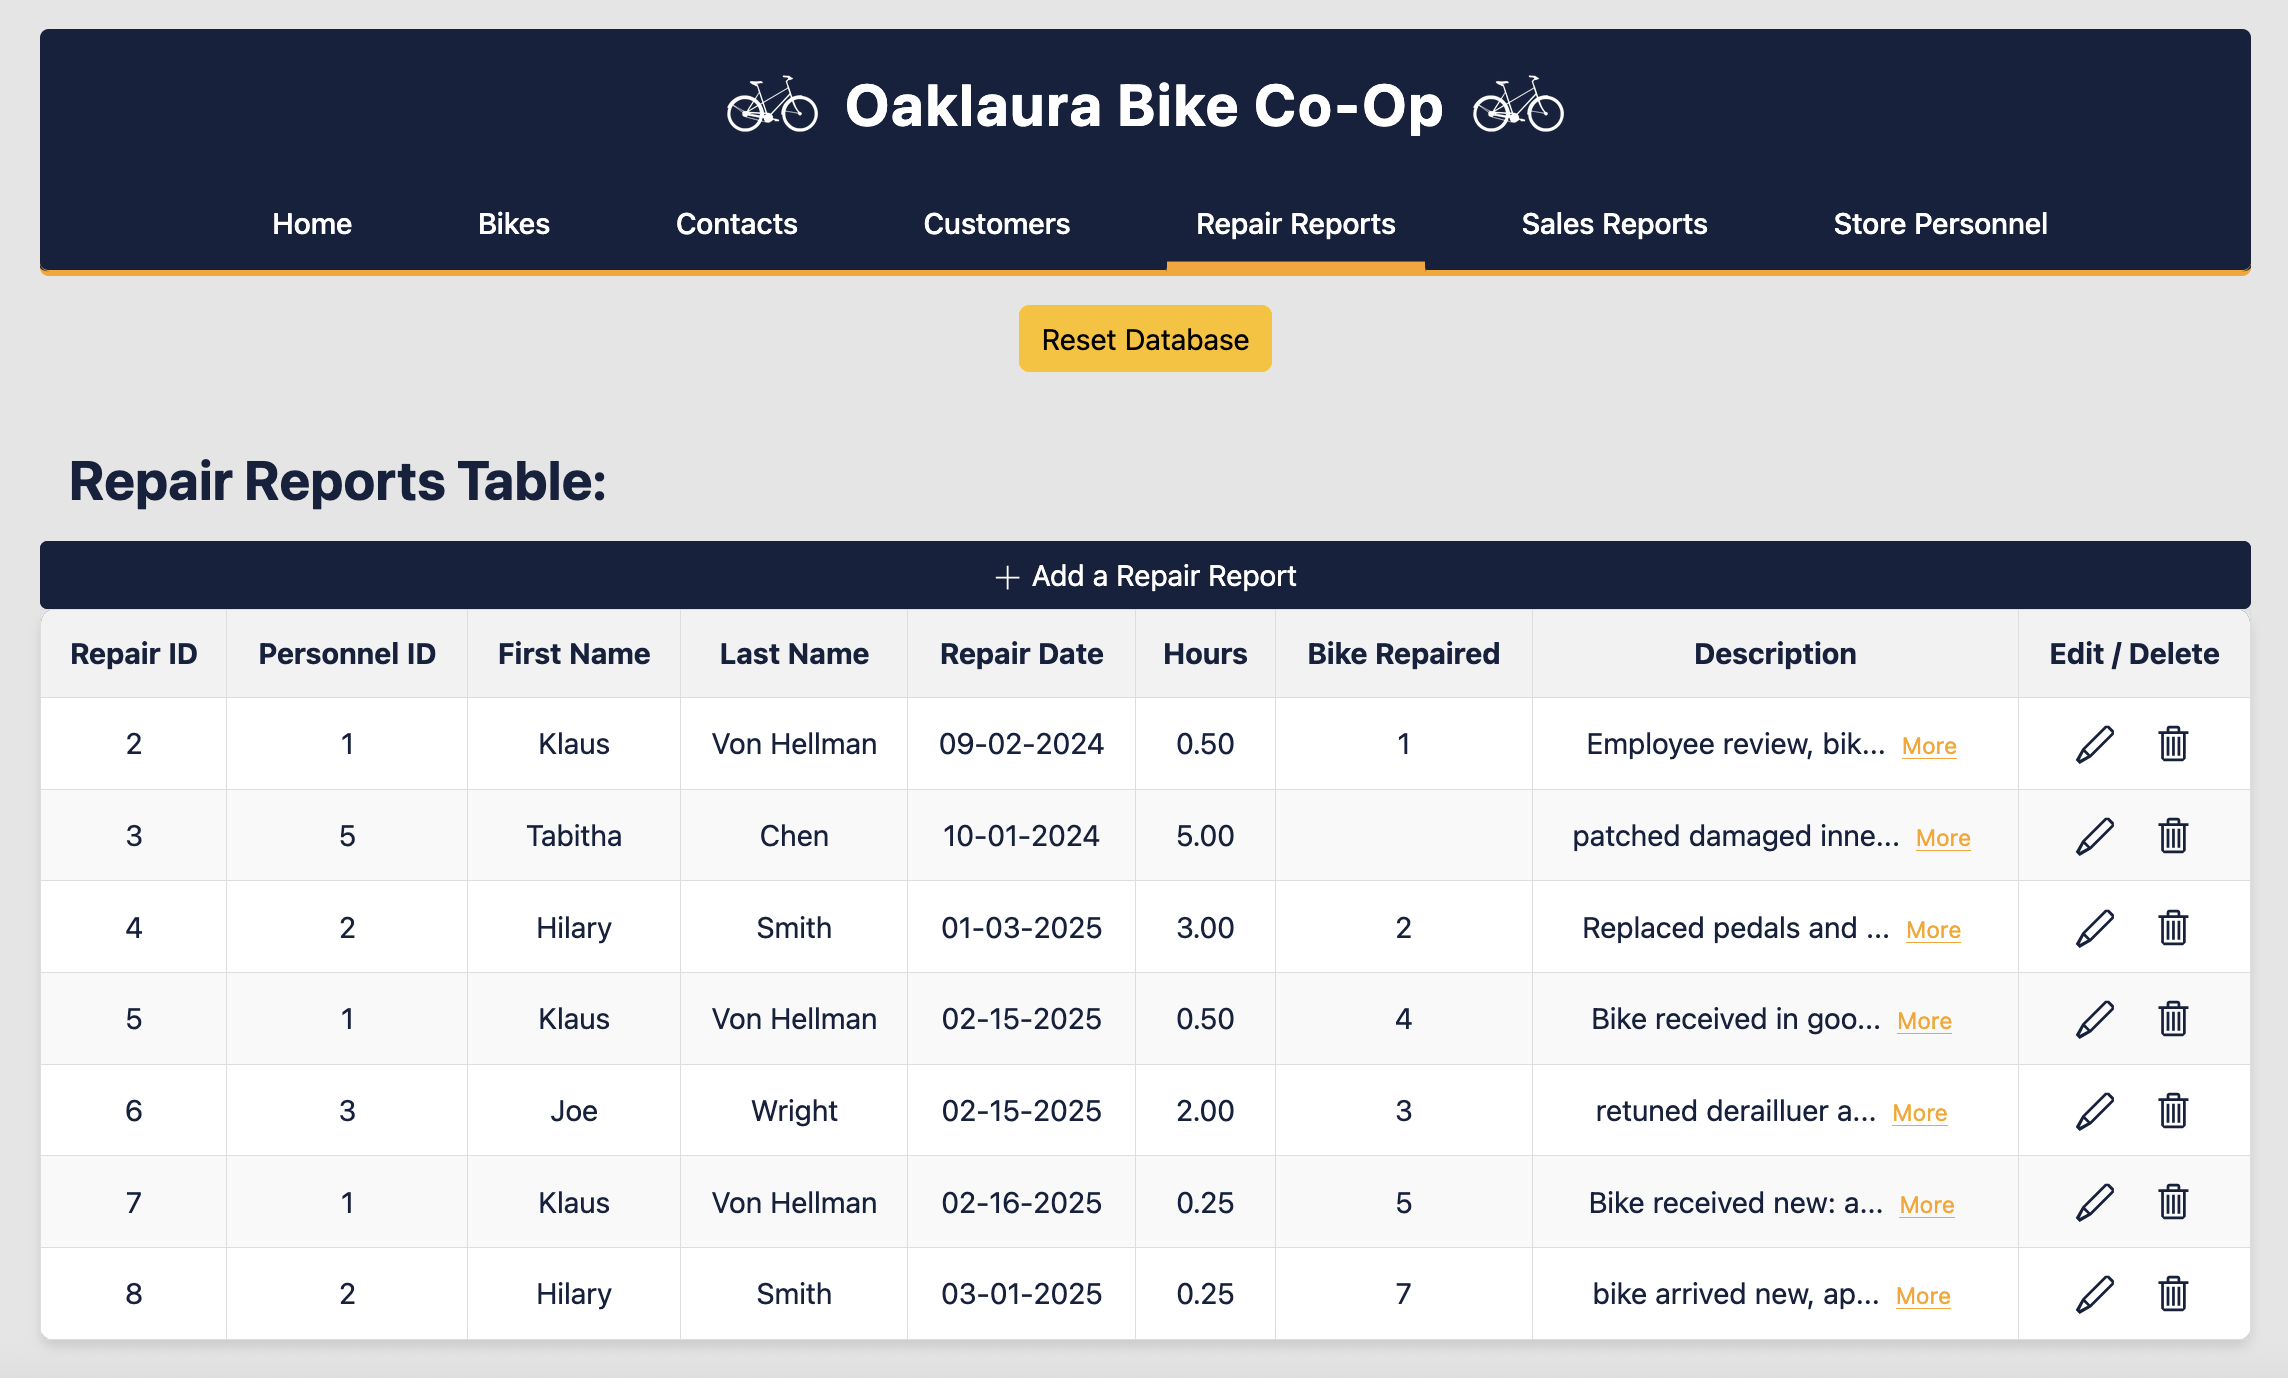
\includegraphics[width=1.0\textwidth]{UI_screenshots/Read_RepairReports.png}
    \label{fig:Read Repair Reports table}
\end{figure}

\begin{figure}[H]
    \centering
    \caption{Read Sales Reports table}
    \vspace{0.2cm}
    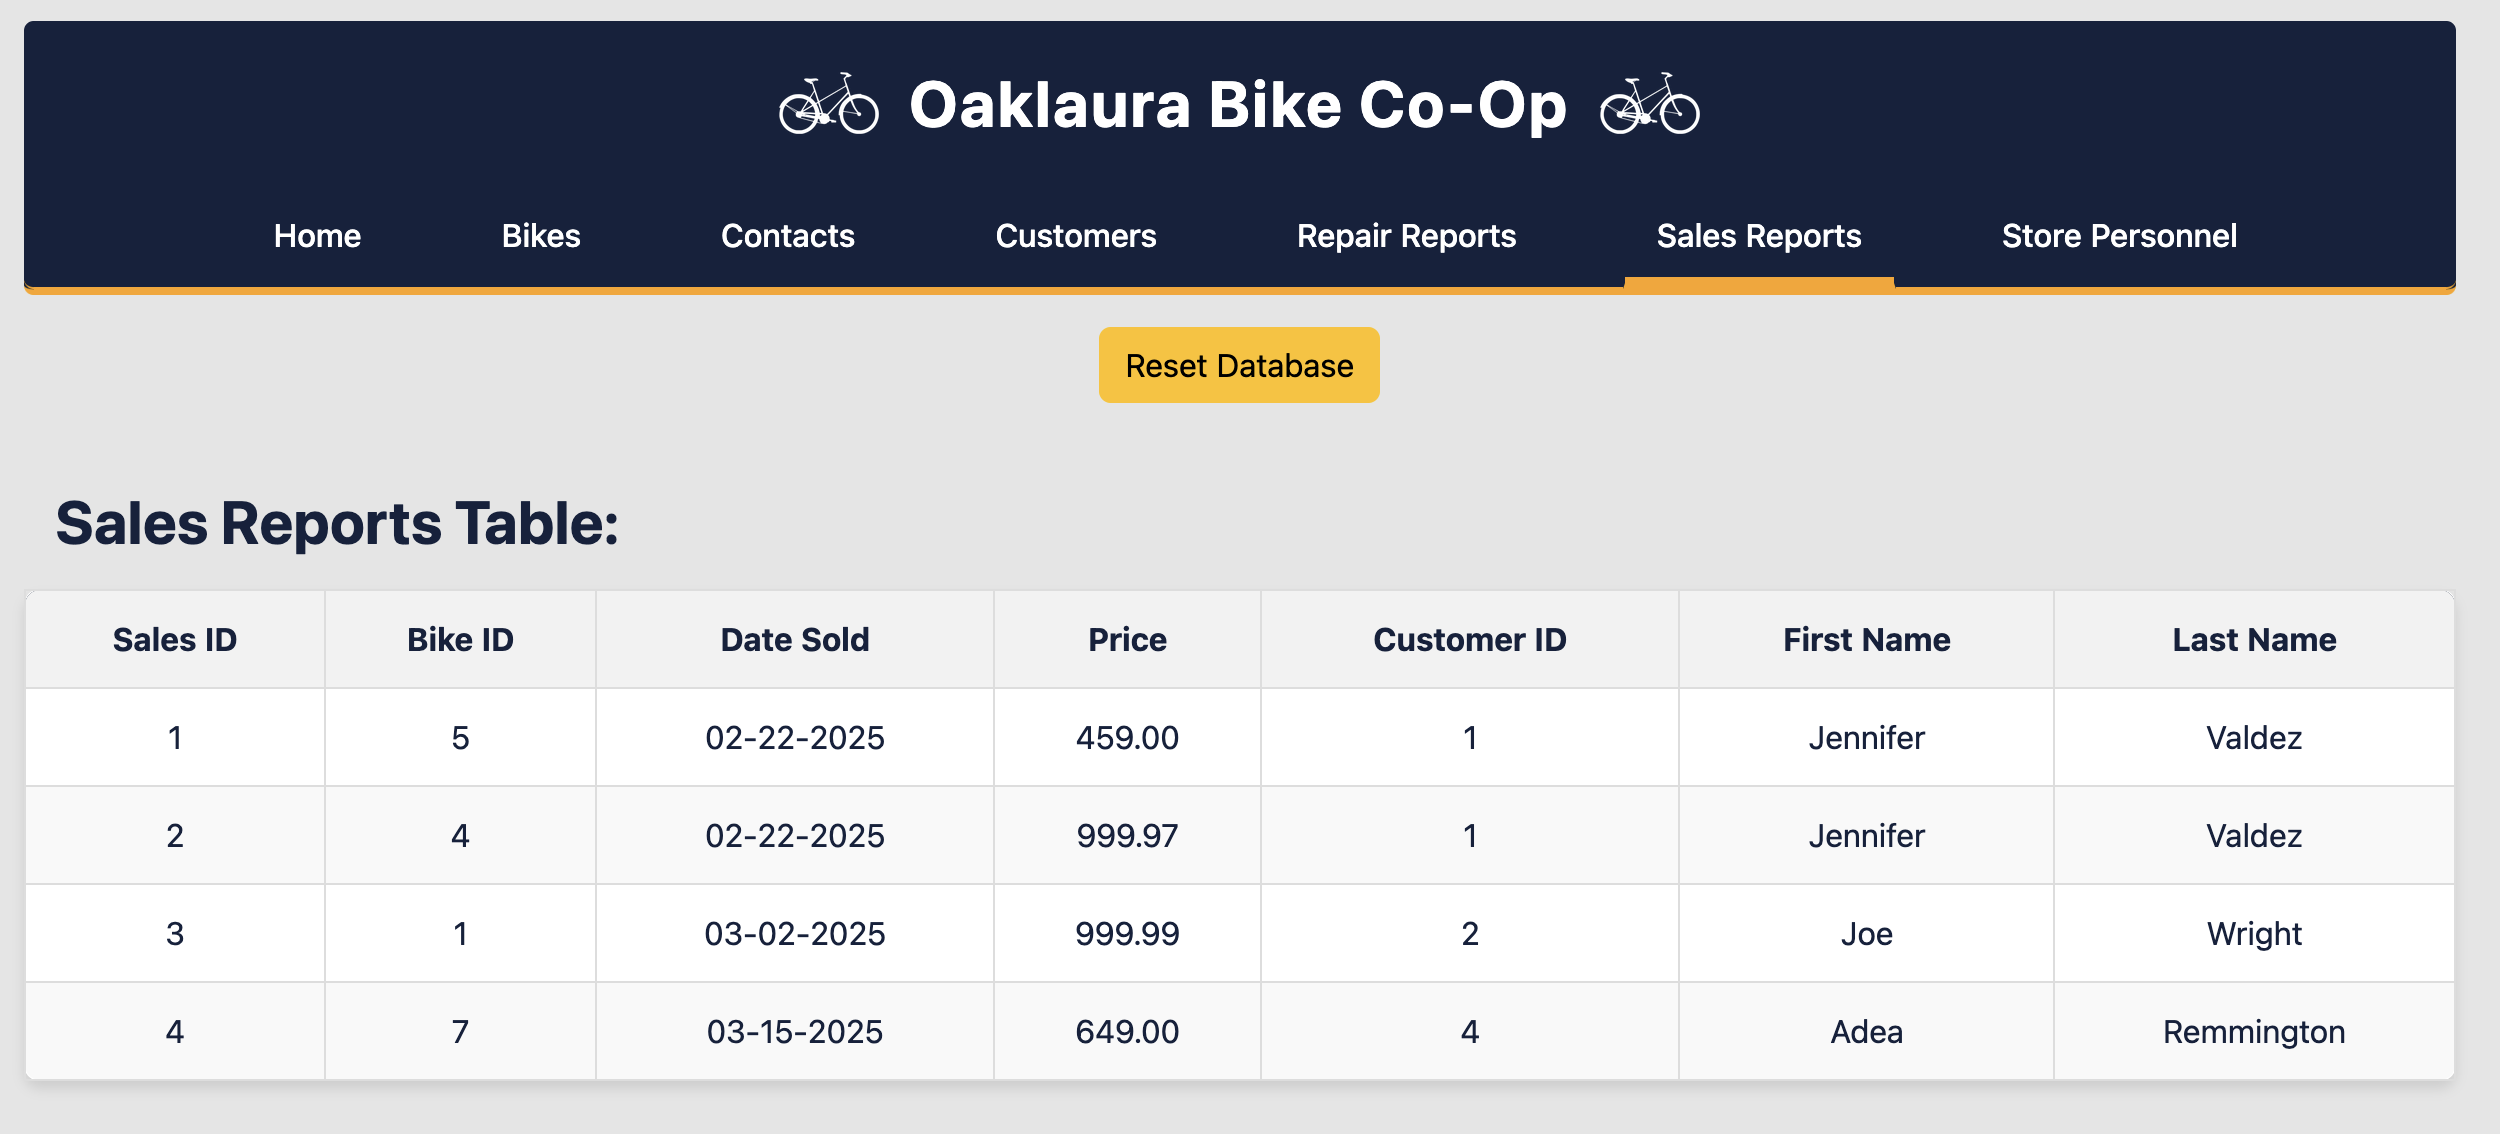
\includegraphics[width=1.0\textwidth]{UI_screenshots/Read_SalesReport_Page.png}
    \label{fig:Read Sales Reports table}
\end{figure}

\begin{figure}[H]
    \centering
    \caption{Read Store Personnel table}
    \vspace{0.2cm}
    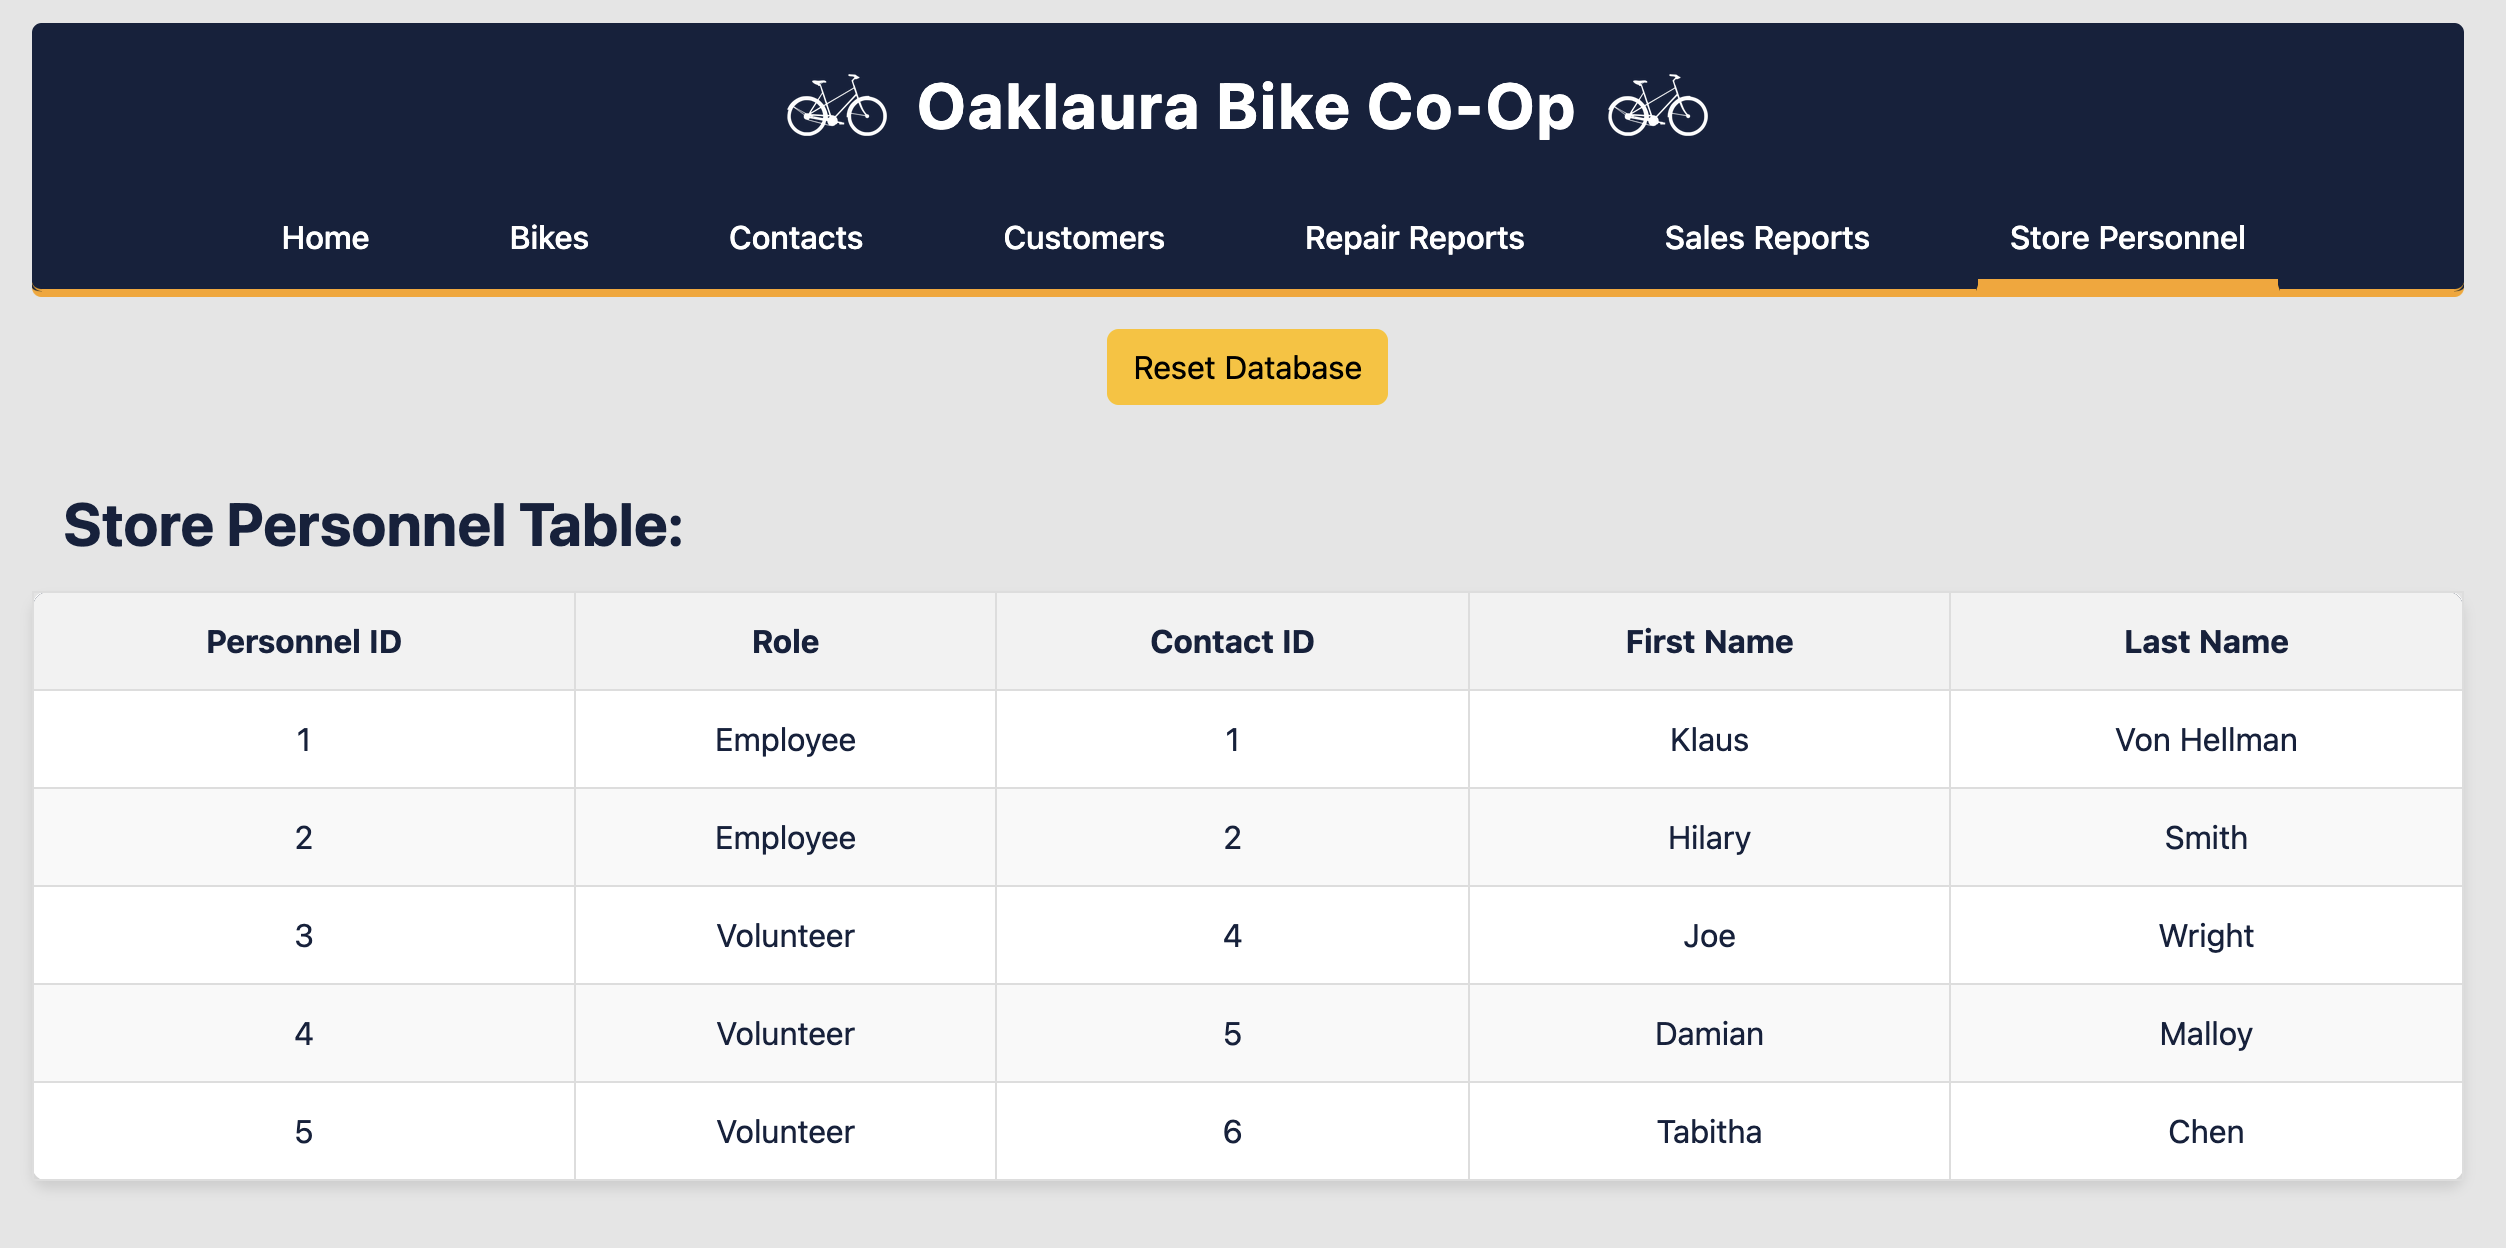
\includegraphics[width=1.0\textwidth]{UI_screenshots/Read_StorePersonnel_Page.png}
    \label{fig:Read Store Personnel table}
\end{figure}

\begin{figure}[H]
    \centering
    \caption{Create M:N Repair Reports table}
    \vspace{0.2cm}
    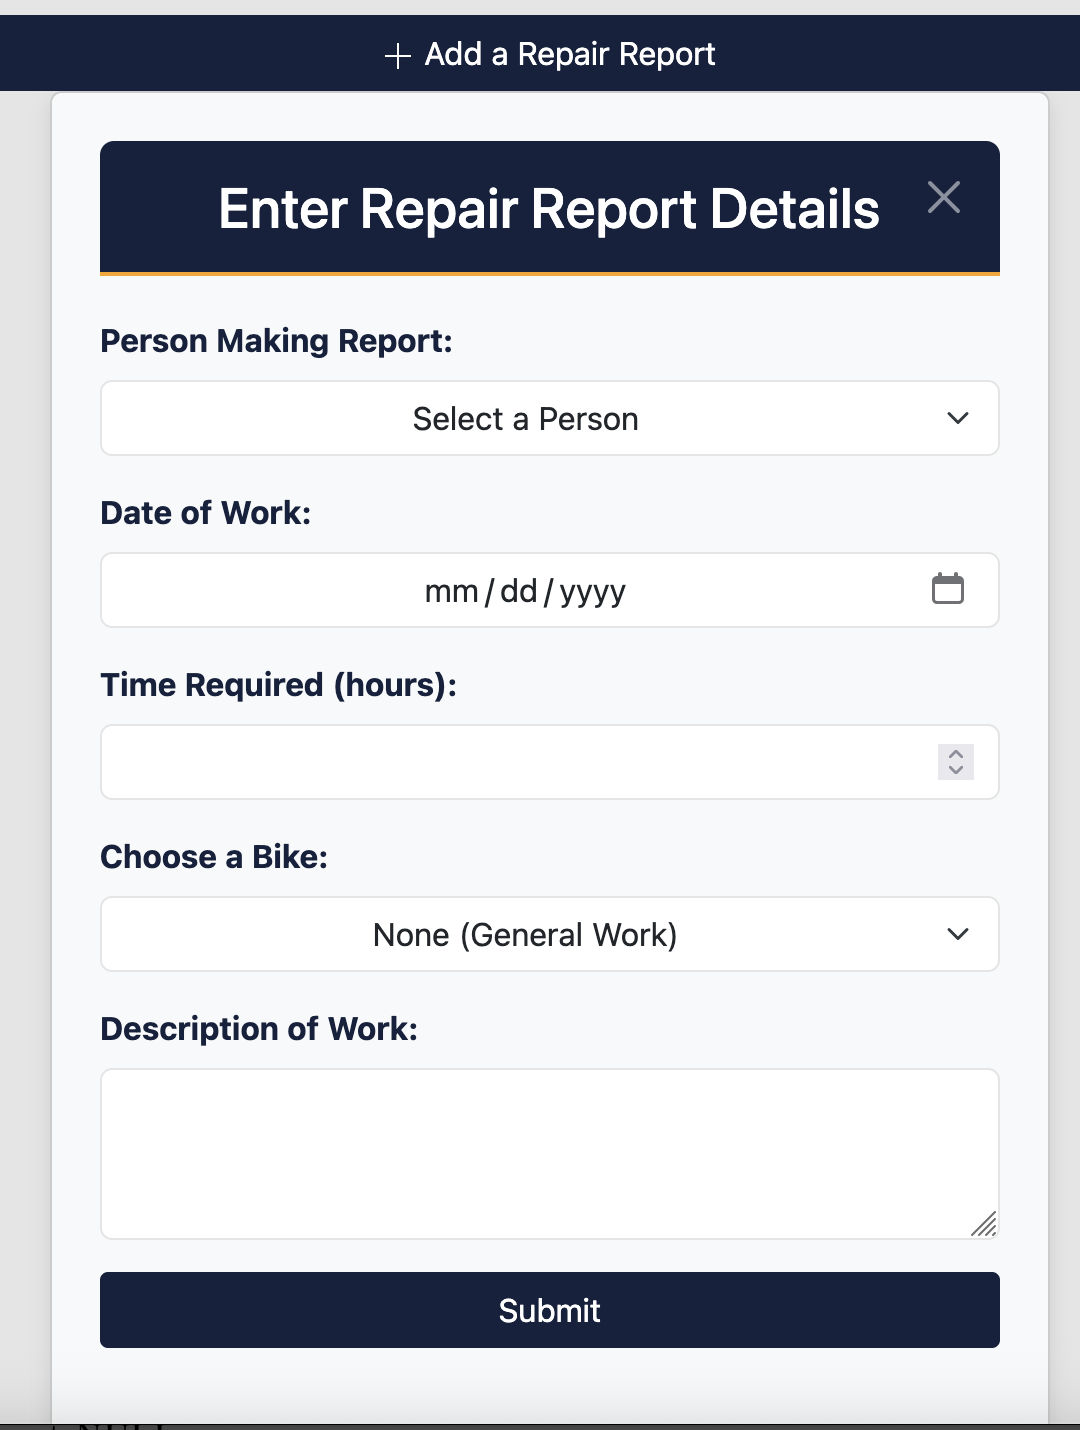
\includegraphics[width=0.5\textwidth]{UI_screenshots/Create_MN_RepairReports.png}
    \label{fig:Create M:N Repair Reports table}
\end{figure}

\begin{figure}[H]
    \centering
    \caption{Update M:N Repair Reports table}
    \vspace{0.2cm}
    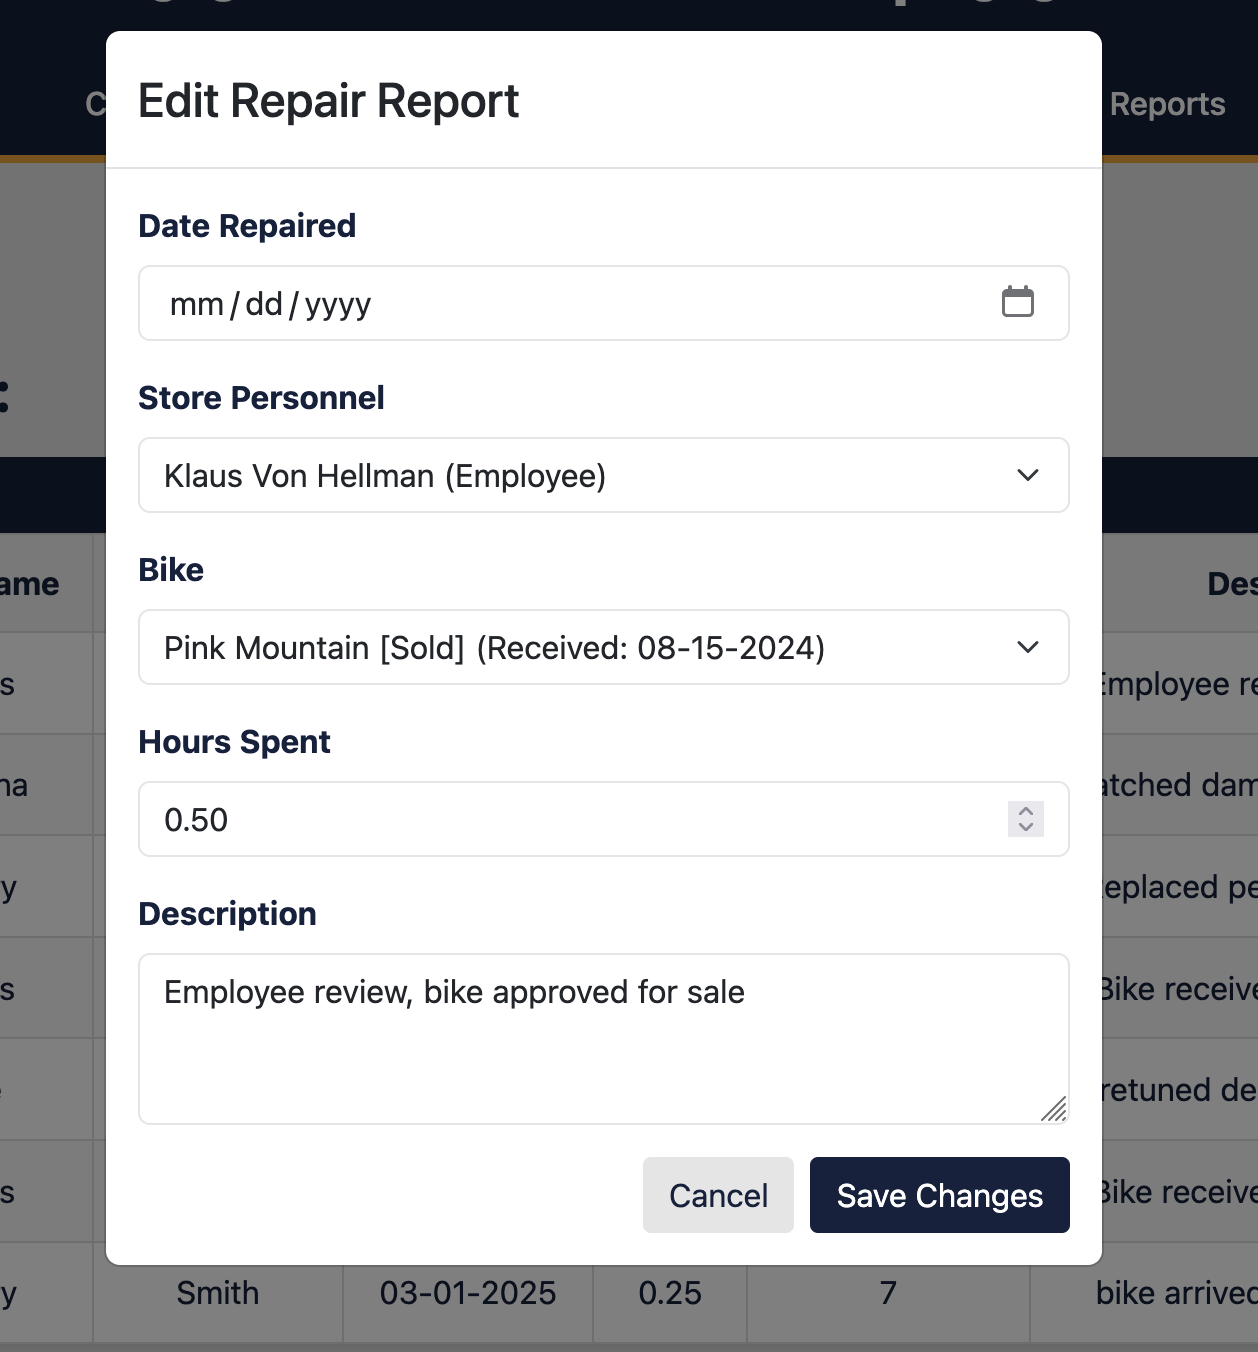
\includegraphics[width=0.5\textwidth]{UI_screenshots/Update_MN_RepairReports.png}
    \label{fig:Update M:N Repair Reports table}
\end{figure}

\begin{figure}[H]
    \centering
    \caption{Delete M:N Repair Reports table}
    \vspace{0.2cm}
    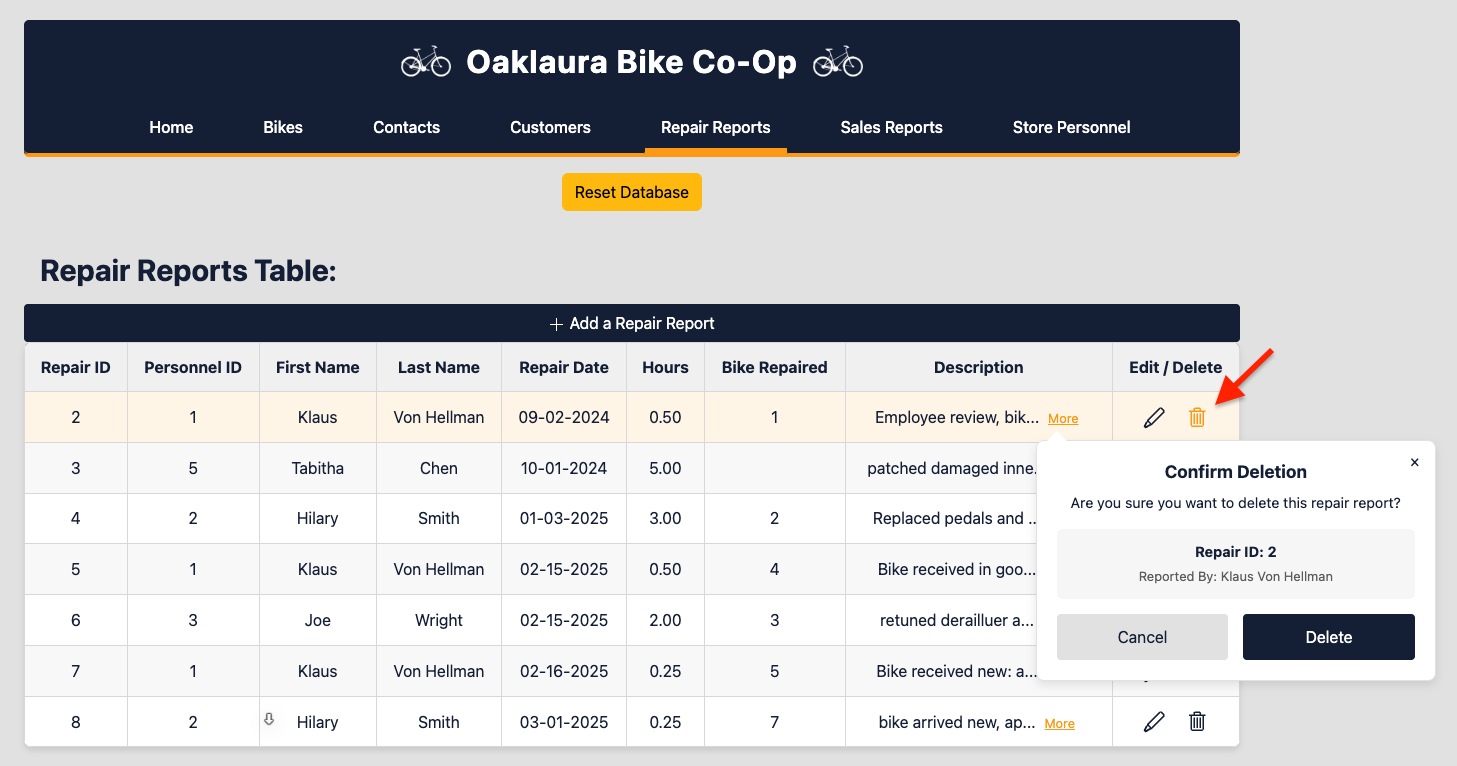
\includegraphics[width=1.0\textwidth]{UI_screenshots/Delete_MN_RepairReports.png}
    \label{fig:Delete M:N Repair Reports table}
\end{figure}

\begin{figure}[H]
    \centering
    \caption{Reset Database}
    \vspace{0.2cm}
    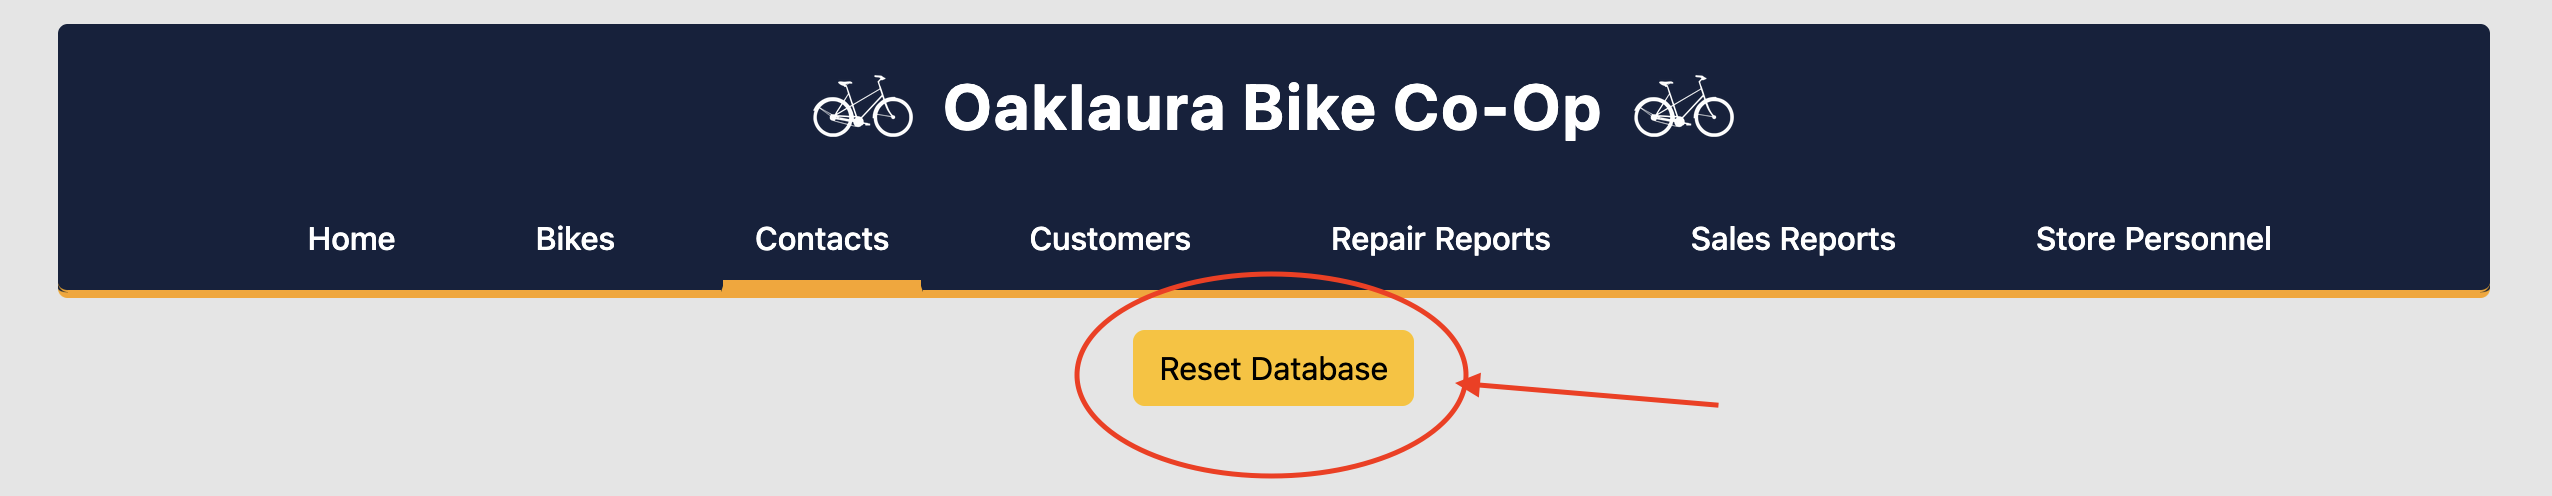
\includegraphics[width=1.0\textwidth]{UI_screenshots/Reset_Database.png}
    \label{fig:Reset Database}
\end{figure}

\begin{figure}[H]
    \centering
    \caption{Reset Database Confirmation}
    \vspace{0.2cm}
    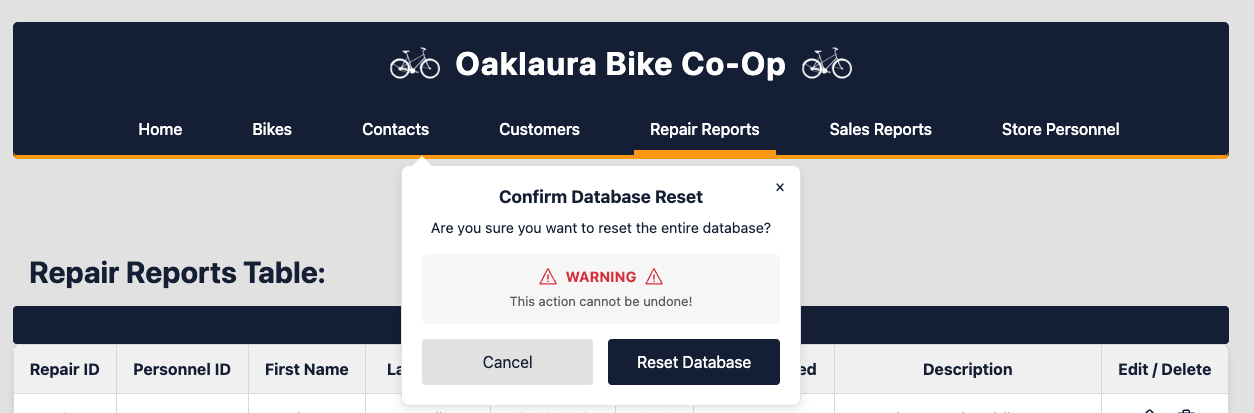
\includegraphics[width=1.0\textwidth]{UI_screenshots/Reset_Database_Confirmation.png}
    \label{fig:Reset Database Confirmation}
\end{figure}

%%%%%%%%%%%%%%%%%%%%%%%%%%%%%%%%%%%%%%%%%%%%%%%%%%%%%%%%%%%%%
%%%%%%%%%%%%%.                   SECTION 8: Citations                       %%%%%%%%%%%%%%%%%%%%%%%%
%%%%%%%%%%%%%%%%%%%%%%%%%%%%%%%%%%%%%%%%%%%%%%%%%%%%%%%%%%%%%
\section{Citations}

\begin{tcolorbox}[colback=secondarycolor, colframe=primarycolor, arc=5mm]
\begin{itemize}
  \item Inspiration for the Bike Co-Op came from The Recyclery, a non-profit bike shop based out of Chicago, IL (last retrieved on 4/9/2025): \href{https://www.therecyclery.org/}{https://www.therecyclery.org/}
  
  \vspace{0.2cm}
  
  \item MySQL workbench was used to create the ERD diagram shown above.
  
  \vspace{0.2cm}
  
  \item The \LaTeX\ template used here was adapted from the Cleese-Assignment template v.2.0 (retrieved on 4/2/2025): \href{https://latextemplates.com/template/cleese-assignment}{https://latextemplates.com/template/cleese-assignment}
  
  \vspace{0.2cm}
  
  \item TeXShop was used for all \LaTeX\ related compilations.
  
  \vspace{0.2cm}
  
  \item All database design work is original.
\end{itemize}
\end{tcolorbox}

\end{document}